\chapter{今日的扩散模型：Score SDE 框架}\label{ch:score-sde}

\epigraph{
    \textit{呈现物理定律只有一种精确的方式，那就是借助微分方程。它们的优势在于具有根本性，并且据我们所知是精确的。
}}{Richard P. Feynman}



到目前为止，我们已经从两个视角研究了扩散模型：变分视角与分数基视角，后者自然地从 EBM 的表述中产生。现在我们迈出下一步，进入\emph{连续时间框架}。其核心是 \emph{Score SDE}，它是将 DDPM 与 NCSN 统一为单一表述的连续极限。这一视角极为强大，因为它以基于微分方程（DE）的、干净而富有原理的描述来扩展离散更新。
在这一视角下，生成退化为随时间求解一个 DE。这使我们能够直接应用数值分析中的工具：例如，基本的 Euler 方法可以模拟其动力学，而更高级的求解器则能改善稳定性与效率。
通过在连续时间下工作，我们还获得了更丰富的数学结构，以及用于理解、分析和改进扩散模型的统一基础。本专著将进一步发展这一视角。






\newpage

\section{Score SDE：其原理}\label{sec:dm-today}
% The use of multiple noise scales has been a crucial ingredient in the success of NCSN and DDPM frameworks. In this section, we introduce the foundation of the \emph{Score SDE}~\citep{song2020score}, which elevates this idea by considering a continuum of noise levels which this continuous-time limit of forward/reverse diffusion model perspective had been pointed out in \citep{sohl2015deep}. Instead of perturbing data using a fixed or finite set of noise magnitudes, \citet{song2020score} propose a formulation in which the data distribution evolves smoothly over time according to an SDE, as the noise level continuously increases. This continuous-time perspective not only unifies prior discrete models, but also enables a principled and flexible framework for generative modeling via continuous-time processes.
\begin{figure}
    \centering
    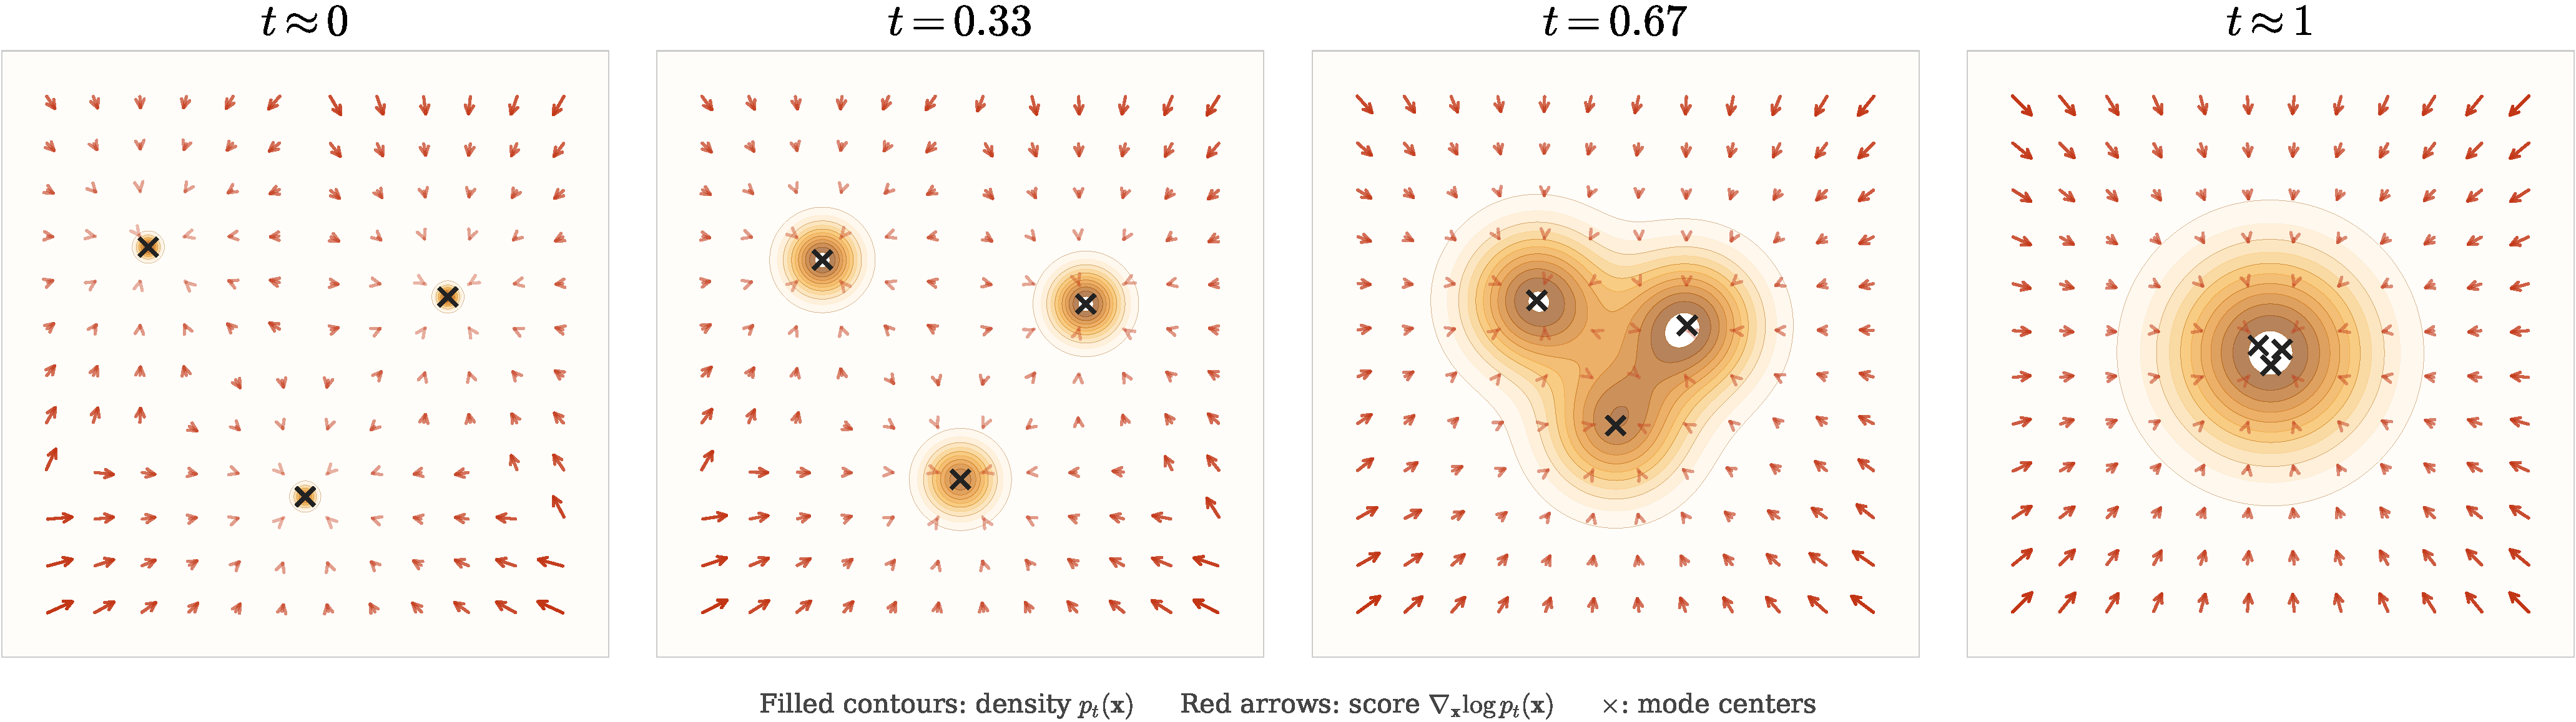
\includegraphics[width=\linewidth]{Images/PartB/score_landscape_2d.pdf}
    \caption{\textbfs{时间依赖分数景观的示意图。}
随着噪声水平增加，受扰密度 $p_t(\rvx)$ 从集中于数据模态附近的多峰分布（数据）演化为宽阔的、几乎单峰的分布（先验）。
相应地，分数场 $\nabla_{\rvx}\log p_t(\rvx)$ 从将样本拉向邻近模态的尖锐局部向量场，变为指向整体质心的平滑全局场。
这一时间依赖的分数场是基于分数的扩散模型（即 Score SDE）所学习的关键对象。 \figcredit{由作者借助 AI 辅助编程绘制。}}
    \label{fig:time-dependent-score}
\end{figure}

% The use of multiple noise scales has been a crucial ingredient in the success of NCSN and DDPM frameworks. In this section, we introduce the foundation of the \emph{Score SDE}~\citep{song2020score}, which elevates this idea by considering a continuum of noise levels. A continuous-time limit of forward and reverse diffusion processes had already been noted by \citet{sohl2015deep}, but \citet{song2020score} make this perspective central by formulating the data evolution as a stochastic/ordinary differential equation, where the noise level increases smoothly over time. This continuous-time formulation not only unifies prior discrete-time models but also provides a principled and flexible foundation for generative modeling by casting it as the problem of solving differential equations.

多种噪声尺度的使用一直是 NCSN 与 DDPM 框架成功的关键因素。在本节中，我们介绍 \emph{Score SDE}~\citep{song2020score} 的基础，它通过考虑连续的噪声水平谱来提升这一思想。前向与反向扩散过程的连续时间极限早已被 \citet{sohl2015deep} 注意到，但 \citet{song2020score} 通过将数据演化表述为一个随机/常微分方程（其中噪声水平随时间平滑增加）使这一视角成为核心。这一表述的核心是\emph{时间依赖的分数函数} $\nabla_{\rvx}\log p_t(\rvx)$：在每个噪声水平~$t$，它指向当前含噪分布~$p_t$ 下密度更高的区域，而正是这个量决定了如何反转扩散过程。如 \Cref{fig:time-dependent-score} 所示，分数场从在小的~$t$ 时尖锐地收敛于各个数据模态，演变为在大的~$t$ 时平缓地指向全局中心。这一连续时间表述不仅统一了此前的离散时间模型，而且为生成式建模提供了富有原理且灵活的基础：在所有噪声水平上学习这一族分数函数，将生成问题归结为求解微分方程的问题。




% \se{might need to properly attribute the 2015 paper, they had a continuous time version there}

% \jcr{The use of multiple noise scales has been central to NCSN and DDPM. In this section we adopt the continuous-time view popularized by the \emph{Score SDE}~\citep{song2020score}, which models a continuum of noise levels via an SDE. A continuous-time perspective predates this:  provided  continuous-time limit and time-reversal perspective of variational-based diffusion model. Building on that foundation, \citet{song2020score} make the reverse-time dynamics explicit in terms of the score $\nabla_{\rvx}\log p_t(\rvx)$, thereby unifying DDPM and SMLD and enabling principled sampling with SDE/ODE solvers. We focus on this score-driven formulation below.
% }

\subsection{动机：从离散到连续时间过程}\label{subsec:scoresde-motivation}

% \se{either reintroduce the symbols, or refer to previous equations. i would probably reintroduce if you expect people to skip chapters}
我们重新审视 NCSN 与 DDPM 的前向噪声注入方案。NCSN 使用一组递增的噪声水平 $\{\sigma_i\}_{i=1}^L$。
每个干净样本 $\rvx_0 \sim p_{\mathrm{data}}$ 被扰动为
\[
\rvx_{\sigma_i} = \rvx_0 + \sigma_i \bm{\epsilon}_i, 
\qquad \bm{\epsilon}_i \sim \mathcal{N}(\bm{0}, \rmI).
\]
DDPM 则通过方差调度 $\{\beta_i\}_{i=1}^L$ 逐步注入噪声\footnote{在 \Cref{sec:ddpm} 中，DDPM 的前向步骤写作 $\rvx_i = \sqrt{1-\beta_i^2}\,\rvx_{i-1} + \beta_i\,\bm{\epsilon}_i$，其中 $\beta_i$ 表示注入噪声的标准差，且 $\alpha_i := \sqrt{1-\beta_i^2}$。在本章及全书中，我们遵循 \citet{song2020score} 的约定，其中 $\beta_i$ 表示注入噪声的方差，故 $\rvx_i = \sqrt{1-\beta_i}\,\rvx_{i-1} + \sqrt{\beta_i}\,\bm{\epsilon}_i$。两种约定通过 $\beta_i^{\textup{(here)}} = \bigl(\beta_i^{\textup{(Ch.\ \ref{ch:variational})}}\bigr)^2$ 相联系，并给出完全相同的动力学。}：
\[
\rvx_i = \sqrt{1 - \beta_i}\, \rvx_{i-1} + \sqrt{\beta_i}\, \bm{\epsilon}_i, 
\qquad \bm{\epsilon}_i \sim \mathcal{N}(\bm{0}, \rmI).
\]

我们在一个离散时间网格上将它们放在一起看待，其中从 $\rvx_t$ 到 $\rvx_{t+\Delta t}$ 的顺序更新形如\footnote{为方便起见，我们互换使用 $\rvx(t)$ 与 $\rvx_t$（其他时间依赖变量亦同理），用以表示时刻 $t$ 的样本。}：
\begin{align*}
    \text{\textbfs{NCSN:}} \,\,
    & \rvx_{t+\Delta t} = \rvx_t + \sqrt{\sigma_{t+\Delta t}^2 - \sigma_t^2} \bm{\epsilon}_t 
    &&\approx \rvx_t + \sqrt{\frac{\diff \sigma_t^2}{\diff t} \Delta t}  \bm{\epsilon}_t \\[0.5em]
    \text{\textbfs{DDPM:}} \,\,
    & \rvx_{t+\Delta t} = \sqrt{1 - \beta(t)\Delta t} \rvx_t + \sqrt{\beta(t)\Delta t} \bm{\epsilon}_t 
    &&\approx \rvx_t - \frac{1}{2} \beta(t) \rvx_t  \Delta t + \sqrt{\beta(t)\Delta t}  \bm{\epsilon}_t,
\end{align*}
其中 $\bm{\epsilon}_t \sim \mathcal{N}(\bm{0}, \rmI)$。有趣的是，这两个噪声注入过程都遵循一个共同的结构模式：
\begin{align}\label{eq:euler-discrete-sde}
    \rvx_{t+\Delta t} \approx \rvx_t + \rvf(\rvx_t, t) \Delta t + g(t) \sqrt{\Delta t}\, \bm{\epsilon}_t,
\end{align}
其中 $\rvf: \mathbb{R}^D \times \mathbb{R} \to \mathbb{R}^D$ 和 $g: \mathbb{R} \to \mathbb{R}$ 由下式给出：
\begin{align*}
    \text{\textbfs{NCSN:}} \quad 
    & \rvf(\rvx, t) = 0, \qquad g(t) = \sqrt{\frac{\diff \sigma^2(t)}{\diff t}} \\[0.5em]
    \text{\textbfs{DDPM:}} \quad 
    & \rvf(\rvx, t) = -\frac{1}{2} \beta(t)\, \rvx, \qquad g(t) = \sqrt{\beta(t)}.
\end{align*}


\begin{figure}
    \centering
    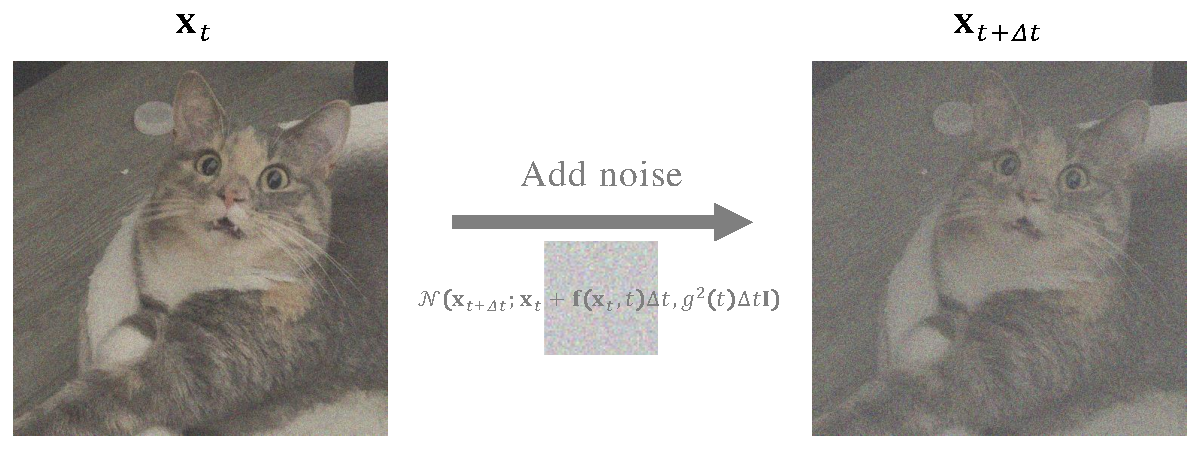
\includegraphics[width=0.9\linewidth]{Images/PartB/sde-forward-noise.pdf}
    \caption{\textbfs{离散时间加噪步骤的示意图。}它以均值漂移项 $\rvf(\rvx_t, t)$ 和扩散系数 $g(t)$ 从 $t$ 到 $t + \Delta t$ 添加噪声。 \figcredit{由作者绘制。}}
    \label{fig:sde-forward-noise}
\end{figure}

该表述对应如下高斯转移：
\begin{align}\label{eq:transition-forward-f-g}
    p(\rvx_{t+\Delta t} |\rvx_t) := \mathcal{N}\!\left(\rvx_{t+\Delta t}; \rvx_t + \rvf(\rvx_t, t)\Delta t,\, g^2(t)\Delta t\, \rmI\right),
\end{align}
其中，在不严格使用记号的情况下，我们将 $\rvx_t$ 视为固定样本，将 $\rvx_{t+\Delta t}$ 视为随机变量。

当 $\Delta t \to 0$（在概念上可理解为准备\emph{无穷多层}噪声）时，离散时间过程收敛为一个沿时间向前演化的连续时间 SDE\footnote{\Cref{eq:transition-forward-f-g} 中的前向核当 $\Delta t\to0$ 时收敛到相应 Itô SDE 的解。完整的严格证明依赖于高级结论，我们将其留待文献中讨论。}：
\begin{align*}
    \diff \rvx(t) = \rvf(\rvx(t), t) \diff t + g(t) \diff \rvw(t),
\end{align*}
其中 $\rvw(t)$ 是标准 Wiener 过程（或布朗运动）。
\rmkb{虽然此处并不需要完整的形式化定义，但 \emph{Wiener 过程}是一个连续时间随机过程 $ \rvw(t) $，它从零开始、具有独立增量，并满足对任意 $ s < t $，增量 $ \rvw(t) - \rvw(s) $ 服从均值为零、方差为 $ t - s $ 的正态分布。它表示独立高斯涨落随时间的累积，虽然它几乎必然连续，却处处不可微。

在一个无穷小时间区间 $[t, t + \diff t]$ 上，Wiener 过程的增量定义为
\[
\diff \rvw(t) := \rvw(t + \diff t) - \rvw(t),
\]
它被建模为均值为零、方差为 $\diff t$ 的高斯随机变量：
\[
\diff \rvw(t) \sim \mathcal{N}(\bm{0}, \diff t \rmI).
\]}

\Cref{app:sde-intro} 提供了 SDE 基础的简要介绍，\Cref{app:Ito} 中则有更深入的讨论。不过，我们可以在概念上按如下方式理解离散与连续表述之间的联系：
\begin{itemize}
    \item $\rvx(t+\Delta t) - \rvx(t) \approx \diff \rvx(t)$，
    \item $\Delta t \approx \diff t$，
    \item $\sqrt{\Delta t} \bm{\epsilon}_t \sim \mathcal{N}(\bm{0}, \Delta t \rmI) \approx \diff \rvw(t)$。
\end{itemize}
一旦指定了漂移项 $\rvf(\rvx,t)$ 与扩散系数 $g(t)$，前向时间 SDE 便自动诱导出一个反向时间 SDE，将终止时的噪声分布传输回数据分布。反向动力学仅包含一个未知项，令人惊讶的是，它正是\emph{每个连续时间水平上的分数函数}。这就把分数匹配确定为训练目标；一旦学得分数，采样便归结为用学得的分数对反向时间 SDE 进行数值积分。


\Cref{sec:scoresde-training-sampling} 给出了实际实现，但我们首先在 \Cref{subsec:forward-sde} 和 \Cref{subsec:reverse-sde} 中考察前向与反向过程的理论基础。




\subsection{前向时间 SDE：从数据到噪声}\label{subsec:forward-sde}
\begin{figure}[th!]
    \centering
    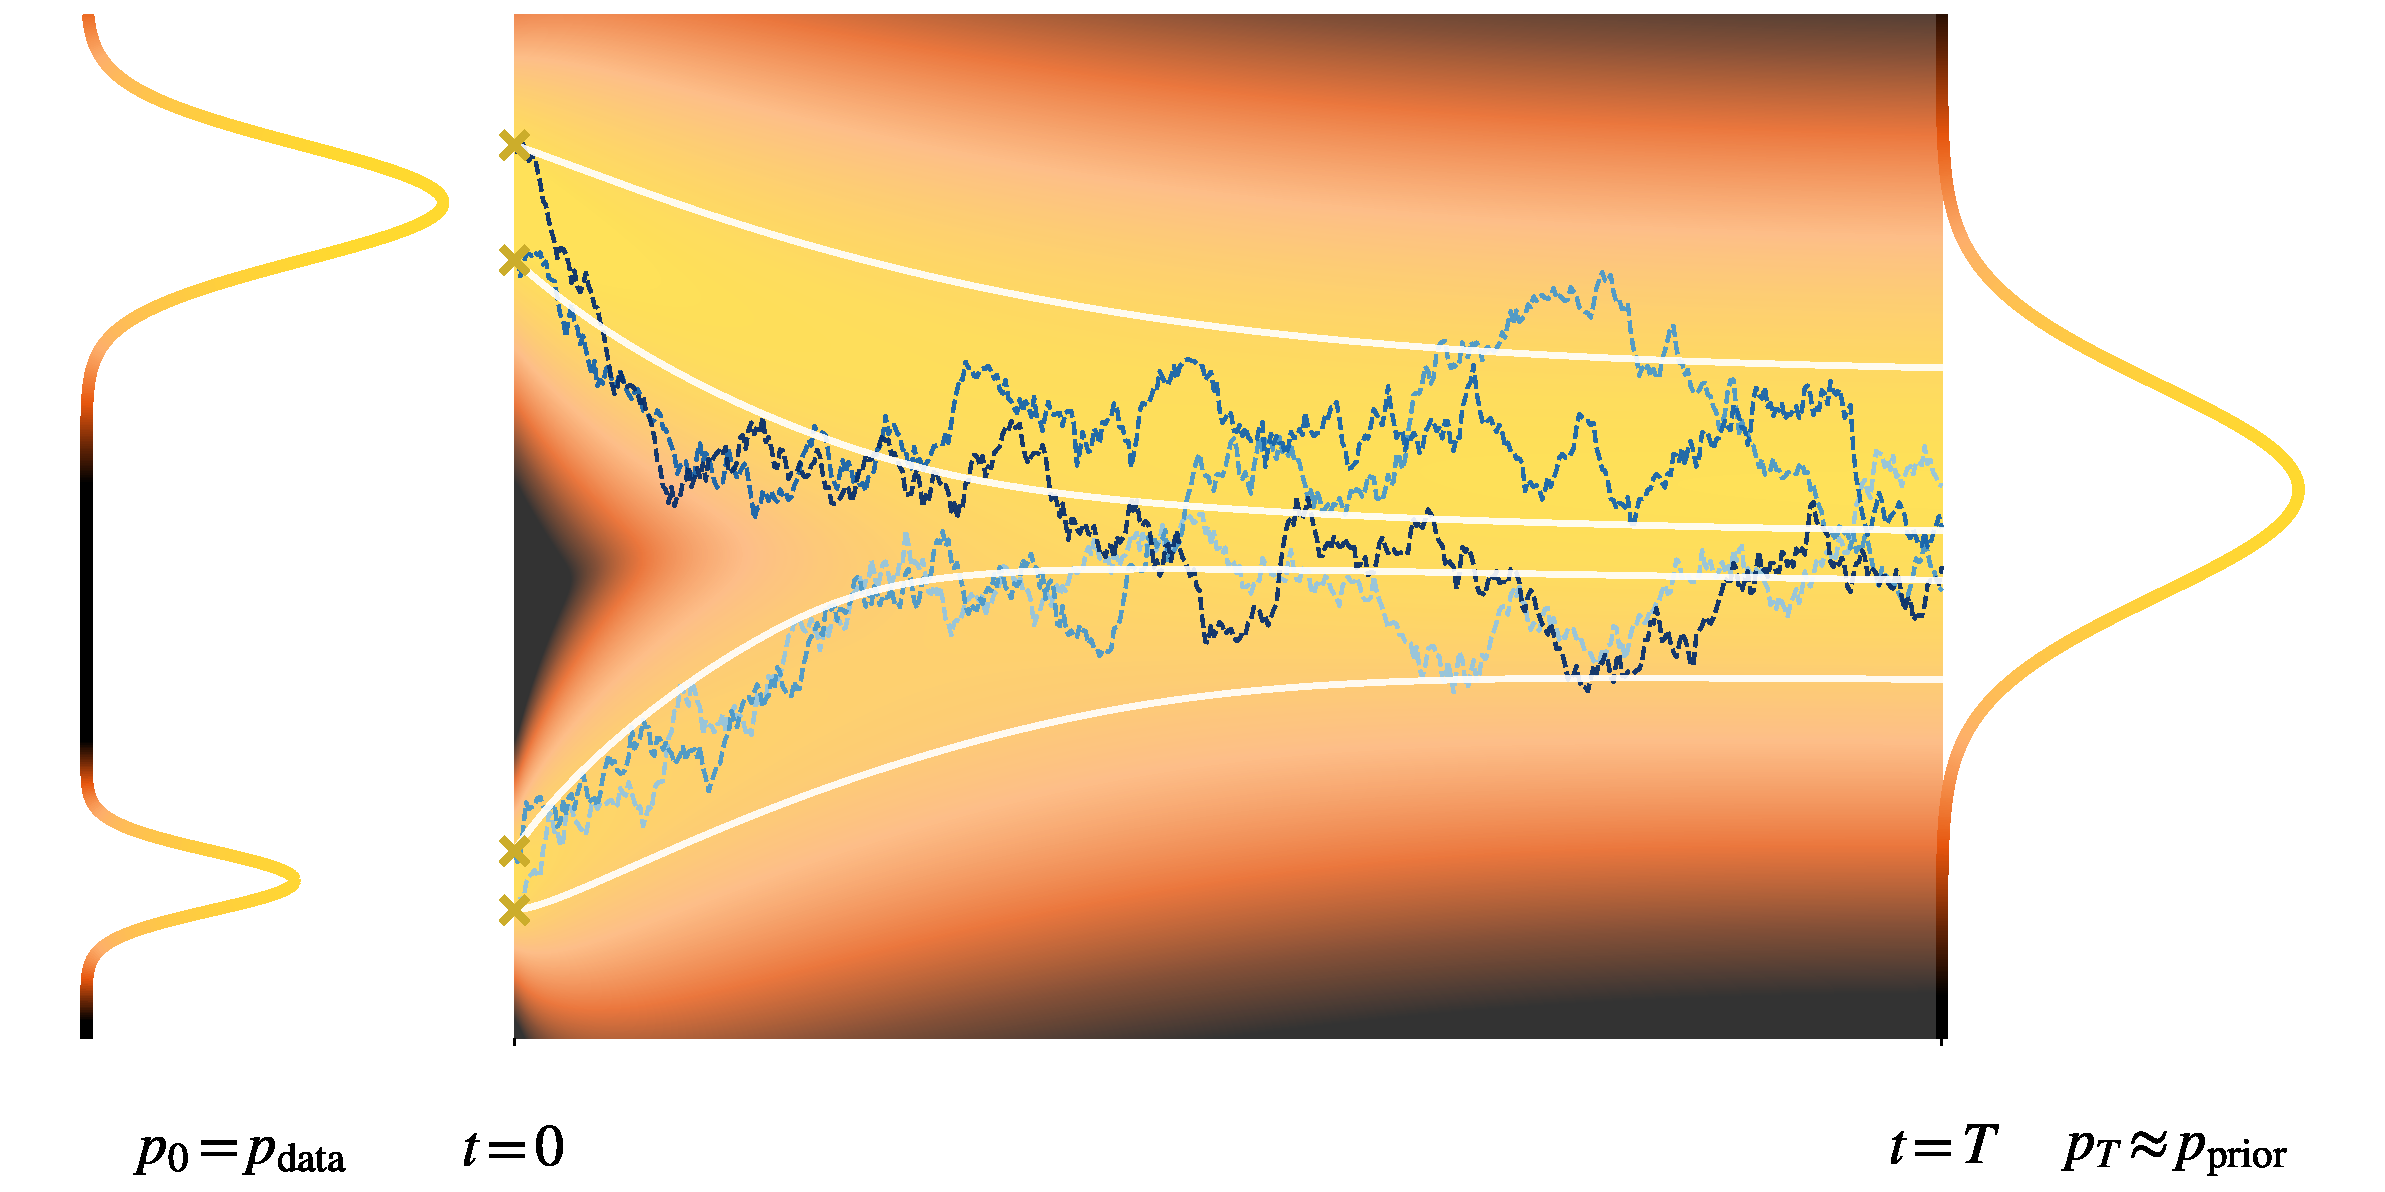
\includegraphics[width=\textwidth]{Images/PartB/forward_sde_ode_trajectories.pdf}
        \caption{\textbfs{（一维）扩散模型中前向过程的可视化。}该过程从复杂双峰数据分布（$p_0 = p_{\mathrm{data}}$）中采样得到的初始点（记为``$\times$''）出发，演化至简单的单峰高斯先验（$p_T \approx p_{\mathrm{prior}}$）。背景热力图展示了不断演化的边缘概率密度 $p_t$，它随时间逐渐变得平滑。图中展示了从 $t=0$ 到 $t=T$ 的样本轨迹，比较了随机前向 SDE 过程（蓝色路径）与其确定性对应物 PF-ODE（白色路径）。注意，PF-ODE 是密度的确定性传输映射，一般并不是从单点出发的样本路径的均值。 \figcredit{由作者绘制。}}

    \label{fig:sde-density-traj}
\end{figure}


借助这一表述，此前基于离散时间的方法，如 NCSN~\citep{song2019generative} 和 DDPM~\citep{sohl2015deep,ho2020denoising}，可以通过定义在区间 $[0, T]$ 上、由前向 SDE 控制的随机过程 $\rvx(t)$ 统一在\emph{连续时间}框架下：
\begin{mdframed}
\begin{equation}\label{eq:sde_forward}
    \diff\rvx(t) = \mathbf{f}(\rvx(t), t) \diff t + g(t) \diff\rvw(t), \quad \rvx(0) \sim p_{\mathrm{data}}.
\end{equation}
\end{mdframed}
这里，$\mathbf{f}(\cdot, t)\colon\mathbb{R}^D\to\mathbb{R}^D$ 是漂移项，$g(t) \in \mathbb{R}$ 是标量扩散系数，$\rvw(t)$ 表示标准 Wiener 过程。我们将其称为\emph{前向 SDE}，它描述了干净数据如何随时间被逐步扰动为噪声。

一旦指定了漂移项 $\mathbf{f}$ 和扩散系数 $g$，前向过程便完全确定，描述了数据变量如何通过注入高斯噪声而被逐步破坏。具体而言，它诱导出两族时间依赖的密度：
\paragraph{扰动核。}
条件分布律
\[
p_t(\rvx_t |\rvx_0)
\]
描述了一个干净数据样本 $ \rvx_0 \sim p_{\mathrm{data}} $ 如何在时刻 $t$ 演化为其含噪对应物 $\rvx_t$。一般而言，\Cref{eq:sde_forward} 中的漂移项 $\rvf(\rvx,t)$ 可以是 $\rvx$ 的任意函数，但一种常见且便于解析的选择是假设它为仿射形式：
\begin{equation}\label{eq:affine-drift}
    \rvf(\rvx,t) = f(t) \rvx, 
\end{equation}
其中 $f(t)$ 是 $t$ 的标量函数，通常取为非正。
在这一结构下，过程在每一时刻都保持高斯性，且条件分布存在通过求解相关的均值--方差 ODE~\citep{sarkka2019applied} 得到的闭式解（另见 \Cref{subsec:scoresde-perturbation-kernel}）。{特别地，
\[
p_t(\rvx_t |\rvx_0) = \mathcal{N} \big(\rvx_t; \rvm(t), P(t)\mathbf I_D\big),
\]
其中
\[
\rvm(t) = \exp \Big(\int_0^t f(u) \diff u\Big) \rvx_0,
\quad
P(t) = \int_0^t \exp \Big(2 \int_s^t f(u) \diff u\Big) g^2(s) \diff s,
\]
初始条件为 $\rvm(0)=\rvx_0$、$P(0)=0$。}

这一显式形式允许我们在给定 $\rvx_0$ 时直接采样 $\rvx_t$，而无需对 SDE 进行数值积分，因此被称为\emph{免仿真}（simulation-free）。NCSN 与 DDPM 都属于这种仿射漂移设定。

在下文中，我们针对任意漂移项 $\rvf(\rvx,t)$ 发展一般理论，但当闭式分析有用时，我们会回到仿射漂移的情形。



\paragraph{边缘密度。}
时间边缘密度 $ p_t(\rvx_t) $ 通过对扰动核积分得到：
\begin{equation}\label{eq:scoresde-oracle-marginal}
    p_t(\rvx_t) := \int p_t(\rvx_t|\rvx_0) p_{\mathrm{data}}(\rvx_0) \diff \rvx_0, \quad \text{with } p_0 = p_{\mathrm{data}}.
\end{equation}

{通过适当地选择系数 $f(t)$ 和 $g(t)$，前向过程逐步添加噪声，直到初始状态的影响被有效遗忘。当 $T$ 变大时，条件分布 $p_T(\mathbf{x}_T |\mathbf{x}_0)$ 不再依赖于 $\mathbf{x}_0$，因为其均值按如下方式演化
\[
\rvm(T) = \exp\!\Big(\int_0^T f(u)\diff u\Big) \mathbf{x}_0  \longrightarrow  \mathbf{0}, \quad \text{as } T\to\infty,
\]
只要 $f(u)$ 非正，从而使指数因子衰减。同时，方差增长并稳定以匹配所选的先验分布。}因此，边缘分布
\[
p_T(\mathbf{x}_T) = \int p_T(\mathbf{x}_T |\mathbf{x}_0) p_{\mathrm{data}}(\mathbf{x}_0)\diff\mathbf{x}_0,
\]
最初表示数据样本上的复杂混合，最终收敛到一个简单的先验 $p_{\mathrm{prior}}$，通常为高斯分布。在这一极限下，
\[
p_T(\mathbf{x}_T) \approx p_{\mathrm{prior}}(\mathbf{x}_T) 
\quad \text{and} \quad 
p_T(\mathbf{x}_T |\mathbf{x}_0) \approx p_{\mathrm{prior}}(\mathbf{x}_T),
\]
于是前向过程将任意数据分布映射为一个易于处理的先验，为反转与生成提供了便利的起点。




\subsection{用于生成的反向时间随机过程}\label{subsec:reverse-sde}



\begin{figure}[th!]
    \centering
    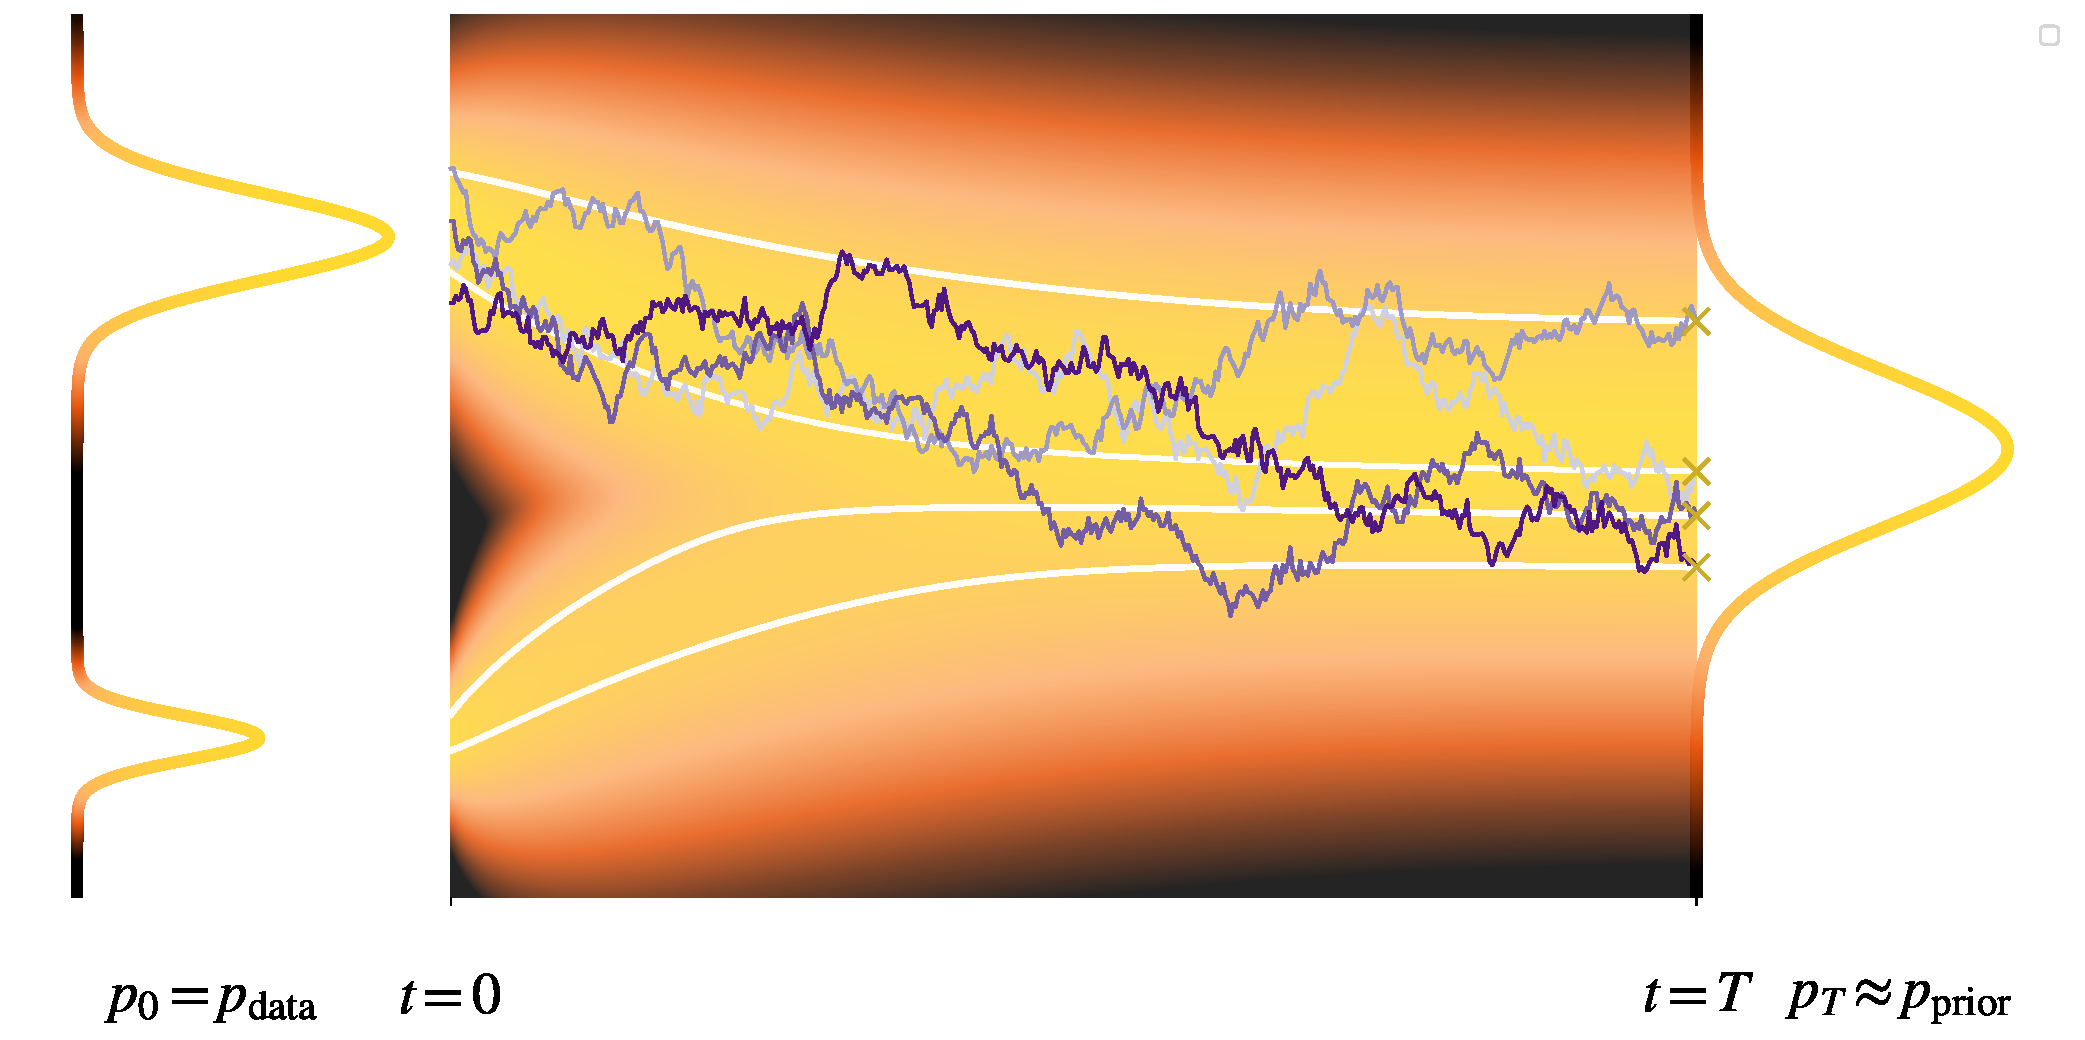
\includegraphics[width=\textwidth]{Images/PartB/reverse_sde_and_ode_trajectories.pdf}
    \caption{\textbfs{用于数据生成的反向时间随机过程的可视化。}
它从 $t=T$ 时由简单先验分布（$p_{\mathrm{prior}}$）中抽取的样本（记为``$\times$''）开始，使用反向 SDE 沿时间向后演化。
所得轨迹在 $t=0$ 处终止，并共同形成目标双峰数据分布（$p_0 = p_{\mathrm{data}}$）。背景热力图展示了概率密度如何从简单的高斯逐步转化为复杂的目标分布。
\figcredit{由作者绘制。}}
    \label{fig:sde-density-back-traj}
\end{figure}
直观上，从噪声生成数据可以通过对前向过程进行``反转''来实现：从先验分布中采样的随机点出发，沿时间向后演化以获得一个生成样本。对于确定性系统（即 ODE），这一想法自然成立。由于不涉及随机性，反转时间仅仅意味着沿与前向过程相同的路径、以相反方向追踪一个点的轨迹\footnote{在技术上，这对应于通过时间翻转替换 $t \leftrightarrow T - t$ 来求解 ODE。}。相比之下，SDE 在每个时间步都引入了随机性，这意味着单个点可以沿许多 plausible 的随机轨迹演化。因此，反转这类过程更为微妙\footnote{朴素地翻转时间并不能得到正确的反向过程。}。

虽然单条随机轨迹不可逆，但一个非凡的洞见是：这些轨迹上的分布是可以被反转的。这由 \citet{anderson1982reverse} 的一个基础结论形式化，它表明前向过程（\Cref{eq:sde_forward}）的时间反演过程 $\{ \bar{\rvx}(t) \}_{t \in [0, T]}$\footnote{我们使用``bar''记号以区分由前向时间 SDE 定义的前向过程 $\{ \rvx(t) \}_{t \in [0, T]}$ 与反向过程 $\{ \bar{\rvx}(t) \}_{t \in [0, T]}$。}本身受一个良定义的 SDE 所控制。这一反向时间过程从 $T$ 演化到 $0$，其动力学由下式给出：
\begin{mdframed}
\begin{align}\label{eq:sde_backward}
\begin{aligned}[t]
    \diff\bar{\rvx}(t) = \left[\mathbf{f}(\bar{\rvx}(t), t) {\color{orange} - g^2(t) \nabla_{\rvx} \log p_t(\bar{\rvx}(t))} \right] \diff t + g(t) \diff \bar{\rvw}(t), \\
    \hfill\bar{\rvx}(T) \sim p_{\mathrm{prior}} \approx p_T.
\end{aligned}
\end{align}
\end{mdframed}
这里，$\bar{\rvw}(t)$ 表示反向时间中的标准 Wiener 过程，定义为 $\bar{\rvw}(t) := \rvw(T - t) - \rvw(T)$。

为了建立对 \Cref{eq:sde_backward} 的直觉，我们在 \Cref{subsec:example-gaussian} 中给出了一个具体例子，采用高斯数据分布与线性--高斯动力学。这一设定在解析上易于处理：仅用基本微积分和线性代数即可直接推导出时间反演公式，而无需援引 \citet{anderson1982reverse} 的一般理论。
% \se{the gaussian linear dynamics system case could be instructive, you can work out the time reversal formula from basic math/linear algebra}

注意，随机性的存在（$g\neq 0$）引入了一个额外的修正项 $ -g^2(t) \nabla_{\rvx} \log p_t(\bar{\rvx}(t))$，它用于解释扩散的影响，并确保反向动力学正确地再现前向 SDE 所诱导的边缘分布演化（见 \Cref{subsec:fpe-sde-ode}）。

\paragraph{从概念上讲，反向过程为何有效？} \Cref{subsec:reverse-sde-reason} 通过将反向时间 SDE 与 DDPM 的变分框架相联系，给出了一个直观的推导（选读但富有洞见）。这里，我们为反向时间动力学如何从噪声中恢复结构化数据提供互补的直觉。


乍看之下，反向时间过程中存在布朗噪声似乎有些矛盾。如果前向扩散将数据扩散为越来越含噪的构型，那么如何通过反转这一过程（尤其是通过 $\bar{\rvw}(t)$ 引入额外随机性的过程）产生集中于数据流形附近的干净、结构化样本，并不清楚。关键在于反向时间 SDE 并不注入任意随机性。扩散项 $g(t)\diff\bar{\rvw}(t)$ 始终与分数驱动的漂移项 $- g^2(t)\nabla_{\rvx}\log p_t(\bar{\rvx}(t))$ 耦合在一起。这两项相互平衡：分数将轨迹引向更高密度的区域，而噪声则引入受控的随机性，使得在不压倒动力学的前提下进行探索。
% \se{refer to langevin?}

为更清楚地看到这一点，回到 \Cref{eq:continuous-langevin} 中的 Langevin 直觉。当 $f(t)\equiv 0$ 时，\Cref{eq:sde_backward} 写作
\[
\diff\bar{\rvx}(t)
= - g^2(t) \nabla_{\rvx}\log p_t\!\big(\bar{\rvx}(t)\big) \diff t
+ g(t)  \diff\bar{\rvw}(t).
\]
通过 $s:=T-t$（从而 $\diff t=-\diff s$）对时间进行前向重参数化，并在分布意义下将布朗运动重新记为 $\diff\bar{\rvw}(t)=-\diff\rvw_s$。记 $\bar{\rvx}_s:=\bar{\rvx}(T-s)$ 与 $\pi_s:=p_{T-s}$，得到
\begin{align*}
    \diff\bar{\rvx}_s
    &= g^2(T-s) \nabla\log \pi_s \big(\bar{\rvx}_s\big) \diff s
    + g(T-s) \diff\rvw_s
    \\&=
2\tau(s) \nabla\log \pi_s\!\big(\bar{\rvx}_s\big) \diff s
    + \sqrt{2\tau(s)} \diff\rvw_s,
    \quad
    \tau(s):=\tfrac{1}{2}g^2(T-s).
\end{align*}
这具有带随时间变化温度 $\tau(s)$、以不断演化的密度 $\pi_s$ 为目标的 Langevin 形式。根据 Tweedie 公式（\Cref{eq:tweedie}），分数方向 $\nabla\log \pi_s$ 在每个时间切片上都指向条件干净信号，因此漂移项持续地``拉回''去噪后的结构。

关键在于，$g(t)$ 沿反向轨迹是\emph{退火}的。起初（$s\approx 0$，即 $t\approx T$），$g(T-s)$ 通常较大，故注入的噪声较强，过程进行广泛的探索。随着 $s$ 增大，$g(T-s)$ 减小，随机项减弱，分数项占据主导，将样本拉入 $\pi_s$ 的高密度区域；到 $s=T$（即 $t=0$）时，轨迹集中于数据流形附近。



% \se{refer to langevin?}

\paragraph{反向时间 SDE 能力概述。}

% \se{i think it's worth saying that solving the reversesde generates sampling, and it's completely determined by the scores (so if we know them, we have all we need)}
令人着迷的是，时间依赖的分数函数
\[
\rvs(\rvx, t) := \nabla_{\rvx} \log p_t(\rvx)
\]
自然地出现在 \Cref{eq:sde_backward} 中。一旦指定了前向系数 $f(t)$ 和 $g(t)$，分数便是反向动力学中唯一剩下的未知量。这突出了它的核心作用：掌握了分数，反向过程便随之确定，而采样归结为用学得的分数对 \Cref{eq:sde_backward} 进行数值积分。

由于 oracle 分数一般没有闭式表达，我们采用 \Cref{ch:score-based} 的方法，训练一个神经网络 $\mathbf{s}_{\bm{\phi}}(\rvx, t)$ 通过分数匹配来逼近它；细节见 \Cref{subsec:sde-train}。将 \Cref{eq:sde_backward} 中的 $\rvs(\rvx, t)$ 替换为 $\mathbf{s}_{\bm{\phi}}(\rvx, t)$ 即可完全确定反向动力学。

生成对应于从 $t = T$ 出发、以 $\rvx_T \sim p_{\mathrm{prior}}$ 为初始值反向求解反向时间 SDE 至 $t = 0$。重要的是，\citet{anderson1982reverse} 证明了前向与反向过程的边缘密度重合，从而确保当 $p_{\mathrm{prior}} \approx p_T$ 时 $t=0$ 处的样本近似服从 $p_{\mathrm{data}}$。我们将在 \Cref{subsec:sde-sample} 中进一步探讨这一点。






\subsection{用于生成的确定性过程（概率流 ODE）}\label{subsec:pf-ode}
 尽管 \Cref{eq:sde_backward} 中的 SDE 引入了随机性并可能提高生成样本的多样性，但仍有一个问题：
\begin{question}
    是否必须使用 \Cref{eq:sde_backward} 中的 SDE 进行采样？
\end{question}

受 \citet{maoutsa2020interacting} 启发，\citet{song2020score} 还引入了一个确定性过程，即一个 ODE，它以与前向 SDE 相同的边缘分布演化样本。该过程 $\{\tilde\rvx(t)\}_{t\in[0,T]}$\footnote{我们使用波浪号以区分与前向及反向时间 SDE 相关联的过程。下文中，为简洁起见我们省略这一记号区分。}，称为\emph{概率流 ODE（PF-ODE）}，由下式给出：
\begin{mdframed}
    \begin{equation}\label{eq:prob_ode_gt}
    \frac{\diff}{\diff t}\tilde\rvx(t) = \mathbf{f}(\tilde\rvx(t), t) - \frac{1}{2} g^2(t) \nabla_{\rvx} \log p_t(\tilde\rvx(t)).
    \end{equation}
\end{mdframed}

与 SDE 的情形类似，可以用学得的逼近替换真实分数，并从 $t = T$ 到 $t = 0$ 积分反向时间 ODE 来生成样本。具体而言，生成样本（PF-ODE 在 $t=0$ 时的解）形如
\[
\tilde\rvx(T) + \int_{T}^{0} \Big[ \mathbf{f}(\tilde\rvx(\tau), \tau) - \frac{1}{2} g^2(\tau)  \nabla_{\rvx} \log p_\tau(\tilde\rvx(\tau)) \Big]   \diff \tau,
\]
其中初始条件 $\tilde\rvx(T) \sim p_{\mathrm{prior}}$。由于该积分没有闭式表达，实际生成依赖于数值求解器（例如 Euler 方法，见 \Cref{eq:euler-maruyama}）。

与反向时间 SDE 相比，PF-ODE 具有两大关键优势：
\begin{itemize}
    \item ODE 可以沿任一方向积分，既可从 $t=0$ 到 $t=T$，也可从 $t=T$ 到 $t=0$，且使用相同的方程表述，只要在所选端点处给定相应的初始条件即可。这种双向性与 SDE 形成对比，后者一般只允许前向时间积分。
    \item 它受益于为 ODE 开发的大量成熟、现成的数值求解器。
\end{itemize}


我们强调，PF-ODE 并非通过简单地移除 \Cref{eq:sde_backward} 中的扩散项得到；值得注意的是，其漂移项中 $\frac{1}{2}$ 这一因子具有原理性的来源。概括地说，\Cref{eq:prob_ode_gt} 来源于这样选择 ODE 的漂移项，使其演化保持与 \Cref{eq:sde_forward} 中前向 SDE 相同的边缘密度。保证这种边缘对齐的底层原理（即 Fokker-Planck 方程~\citep{oksendal2003stochastic}）将在下一节中详述。


\clearpage
\newpage



\section{前向/反向时间 SDE 与 PF-ODE 中的边缘分布匹配}\label{subsec:fpe-sde-ode}
\begin{figure}[th!]
% \vspace{-0.1cm}
    \centering
    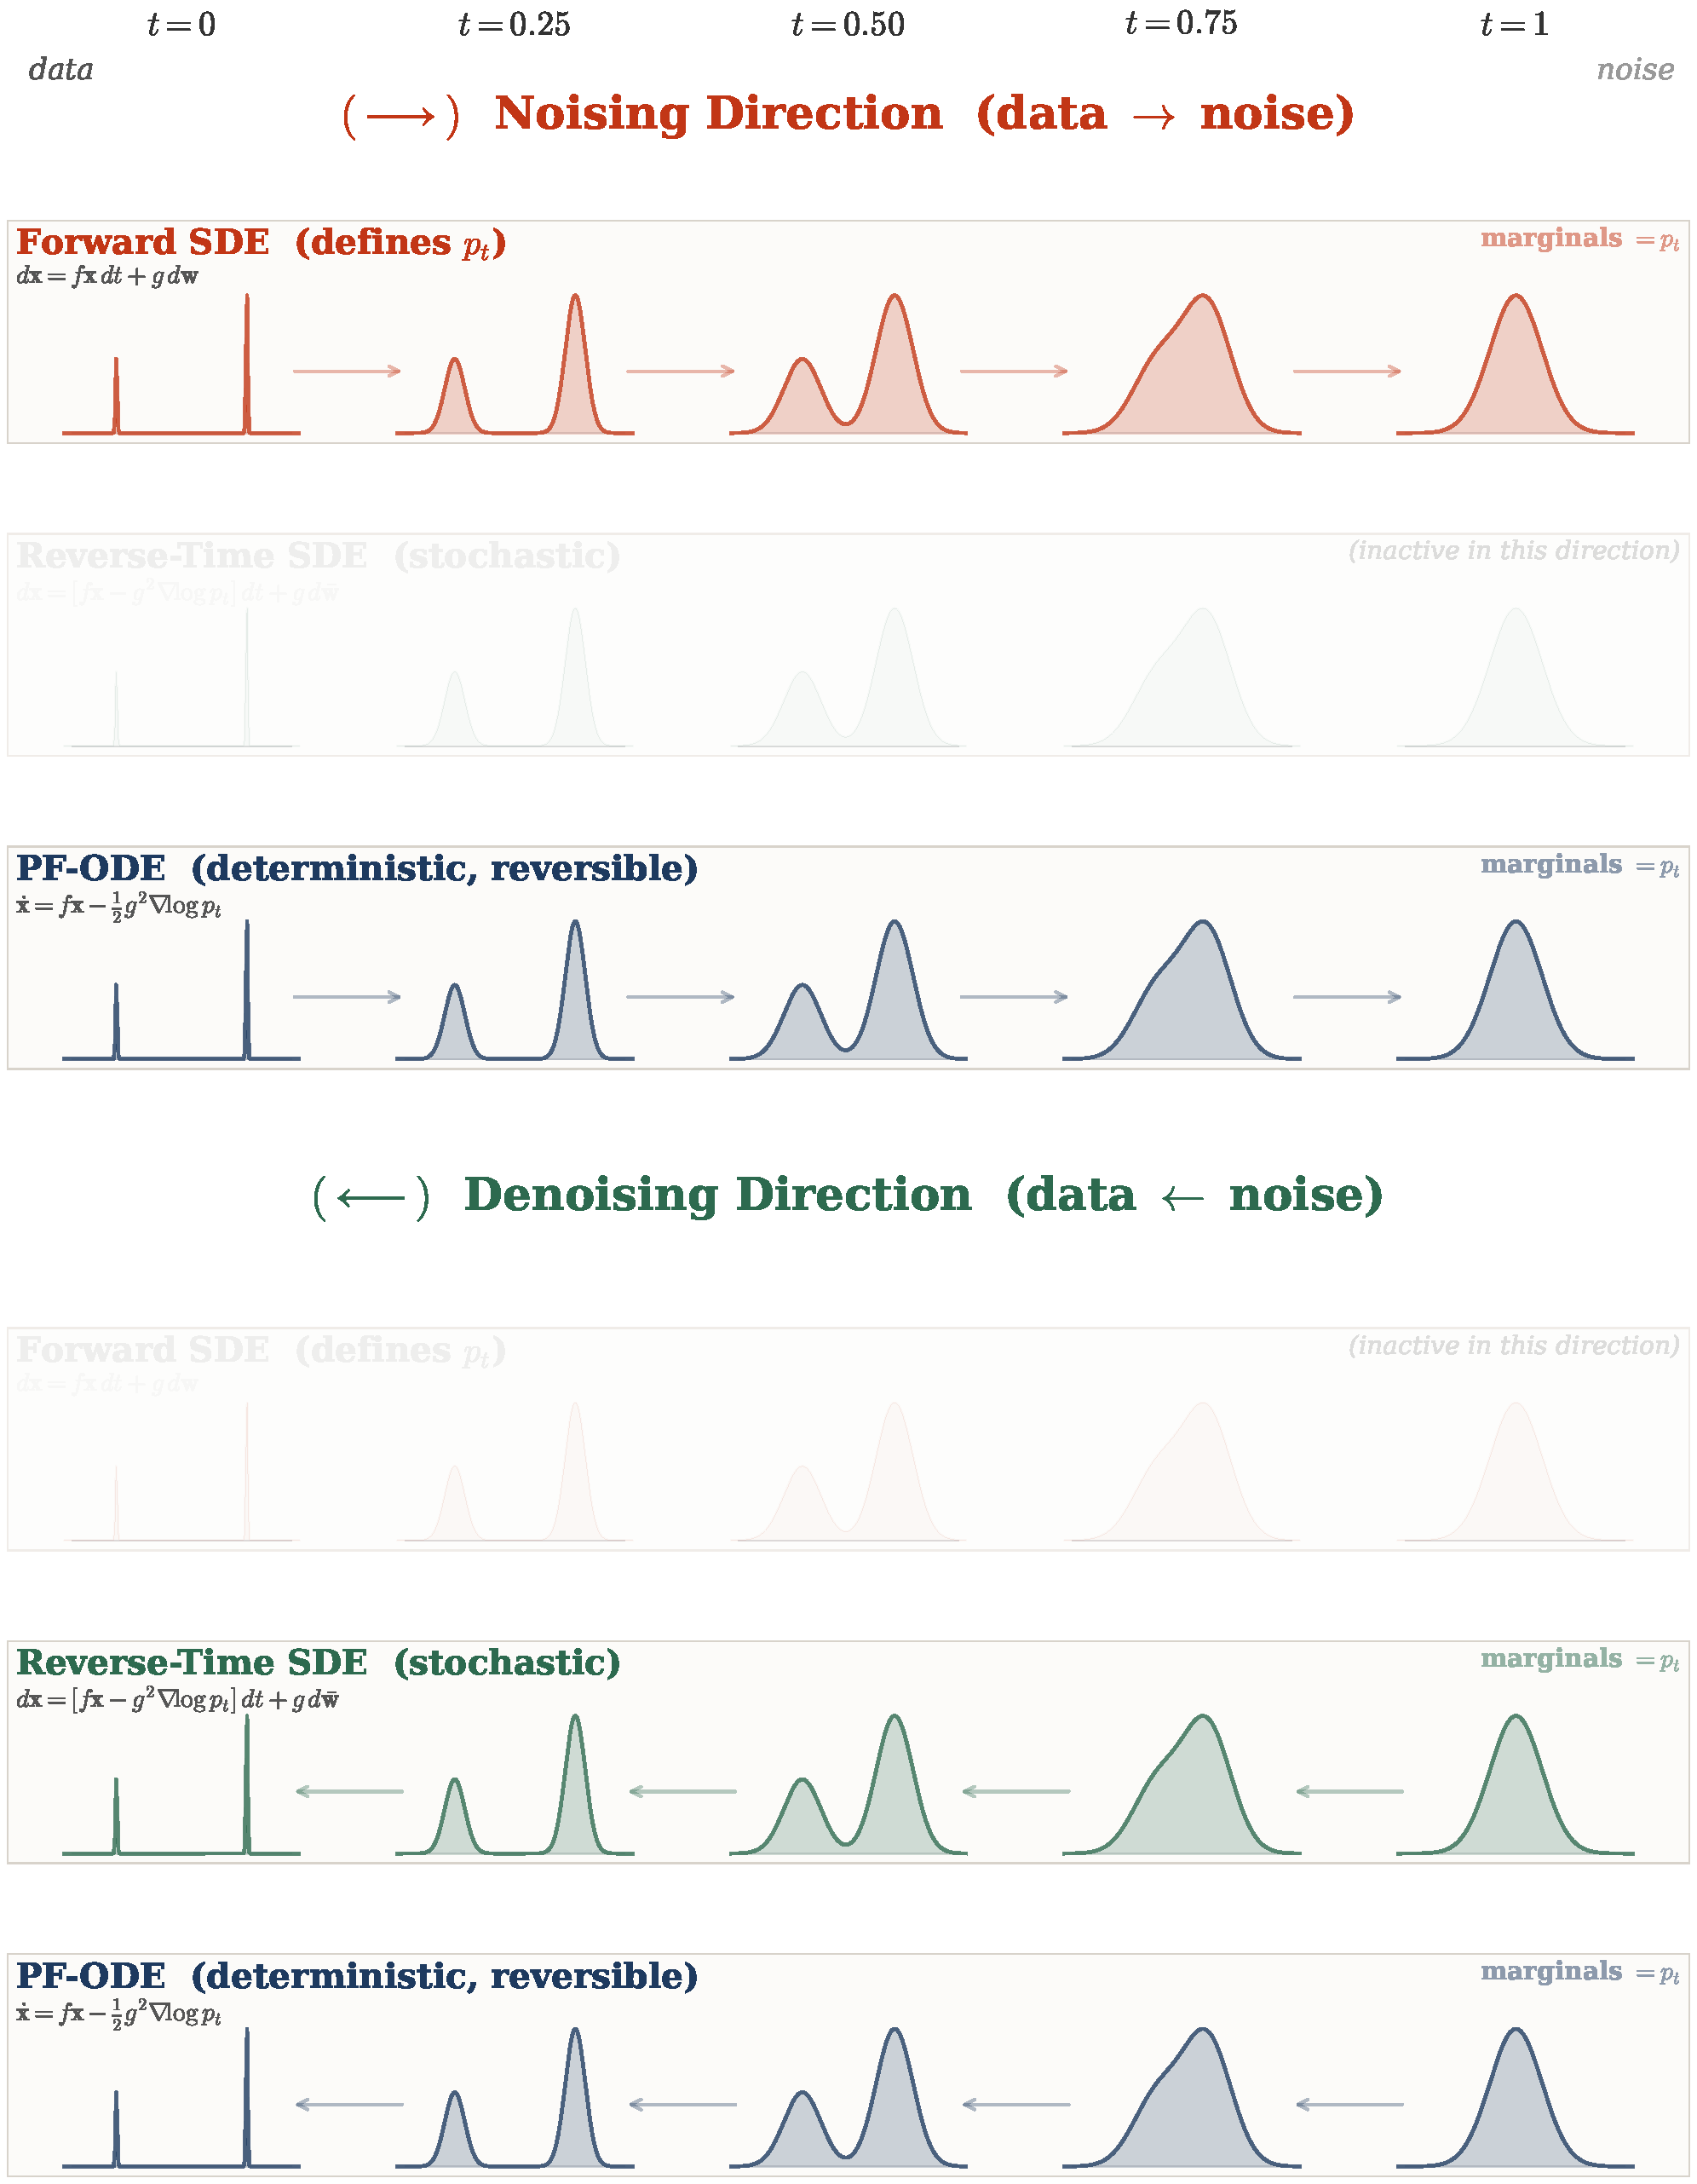
\includegraphics[width=\linewidth]{Images/PartB/score_sde_three_dynamics.pdf}
\caption{\textbfs{三种共享相同边缘分布 $p_t$ 的动力学。}
前向 SDE 作为锚定参考，通过将数据扩散为高斯先验来定义边缘分布 $p_t$。
反向时间 SDE 与 PF-ODE 产生相同的边缘分布，这由 Fokker-Planck 方程保证，同时通过分数 $\nabla \log p_t$ 沿去噪方向移动。
上方面板展示了加噪过程，由前向 SDE 给出，或在边缘层面等价地由沿时间正向运行的 PF-ODE 给出。
下方面板展示了去噪过程，由反向时间 SDE 或沿时间反向运行的 PF-ODE 给出。
PF-ODE 同时出现在两个面板中，因为它是确定性且时间可逆的。
\figcredit{由作者借助 AI 辅助编程绘制。}}
    \label{fig:score-sde-three-dynamics}
    \vspace{-2cm}
\end{figure}
本节中，我们将 \emph{Fokker-Planck 方程}作为支配扩散模型的核心原理加以介绍。它描述了概率密度在含噪动力学下如何演化，并在存在随机性时充当变量替换公式的自然类比（见 \Cref{app:continuity}）。从定义边缘分布 $p_t$ 的前向扩散过程出发，我们解释反向时间 SDE 与 PF-ODE 是如何被设计以再现相同的边缘分布族的。随后，我们通过一个高斯例子使这一原理具体化，在该例子中可以显式、直接地计算出反向时间 SDE 与 PF-ODE。




% \begin{center}
% % \vspace{-0.2cm}
% \includegraphics[width=0.67\linewidth]{Images/PartB/density_evolution_3d_orange.pdf}
%     \captionof{figure}{\textbfs{(2D) Temporal evolution of the marginal density $p_t$.} The forward SDE has $\mathbf{f} \equiv \mathbf{0}$ and $g(t) = \sqrt{2t}$ on $[0,T]$. It starts with $p_0 = p_{\mathrm{data}}$ a two-mode Gaussian mixture and ends at $p_T \approx p_{\mathrm{prior}} := \mathcal{N}(\mathbf{0}, T^2 \mathbf{I})$.  The temporal-spatial evolution of $p_t$ follows the Fokker-Planck equation.
% }
%     \label{fig:fpe-density}
% \end{center}
\subsection{确保边缘密度对齐的 Fokker-Planck 方程}
扩散模型中的一个核心概念是，\emph{不同的过程可以导致相同的边缘分布序列}（我们将在本小节后面加以说明）。
 目标是构造一个通过在时间上（尤其在 $t=0$ 处）对齐边缘分布从而将 $p_{\mathrm{prior}}$ 变换为 $p_{\mathrm{data}}$ 的过程。过程的具体形式是次要的，只要它是易于处理的并且允许高效采样。这自然引出一个根本问题：


\begin{question}
我们如何确保不同的过程产生相同的边缘分布？
\end{question}



回到我们的设定，一旦前向 SDE 被指定，它便定义了边缘密度从 $p_{\mathrm{data}}$ 到 $p_{\mathrm{prior}}$ 的演化。反向时间 SDE 与 PF-ODE 随后被构造出来，使其轨迹所产生的边缘分布与前向过程的边缘分布精确匹配。这种对应关系的关键在于 Fokker–Planck 方程，它支配着边缘密度在扩散过程下的演化。\Cref{fig:score-sde-three-dynamics} 给出了一个图示。下面的定理~\citep{anderson1982reverse,song2020score} 建立了这一联系的基础：
\thmp{Fokker–Planck 方程确保边缘分布对齐}{fpe}{设 $\{\rvx(t)\}_{t\in[0,T]}$ 随前向 SDE 演化
\[
\diff \rvx(t) = \rvf(\rvx(t),t)\diff t + g(t)\diff \rvw(t),
\]
初始条件为 $\rvx(0)\sim p_0 = p_{\mathrm{data}}$。则其边缘密度 $p_t$ 满足 Fokker–Planck 方程
\begin{align}\label{eq:fp_general}
\begin{aligned}
    \partial_t p_t(\rvx)
    &= - \nabla_{\rvx} \cdot\bigl[\rvf(\rvx,t) p_t(\rvx)\bigr]
       + \tfrac12 g^2(t) \Delta_{\rvx} p_t(\rvx)\\
    &= - \nabla_{\rvx} \cdot\bigl[\rvv(\rvx,t) p_t(\rvx)\bigr],
\end{aligned}
\end{align}
其中 $\Delta_{\rvx}$ 表示拉普拉斯算子，且
\[
 \rvv(\rvx,t)
 := \rvf(\rvx,t)
   -\tfrac12 g^2(t) \nabla_{\rvx}\log p_t(\rvx).
\]
那么，PF-ODE 与反向时间 SDE 都产生相同的边缘分布族 $\{p_t\}_{t \in [0, T]}$，其中后者沿反向时间演化：
\begin{enumerate}
  \item[\textup{(i)}] \emph{PF-ODE} $\{\tilde\rvx(t)\}_{t\in[0,T]}$
  \[
    \frac{\diff \tilde\rvx(t)}{\diff t}
    = \rvv(\tilde\rvx(t),t),
  \]
  若以 $\tilde\rvx(0)\sim p_0$ 为初始值并沿 $t$ 正向运行，或等价地以 $\tilde\rvx(T)\sim p_T$ 为初始值并沿 $t$ 反向运行，则对所有 $t\in[0,T]$ 都有边缘分布 $\tilde\rvx(t)\sim p_t$。

  \item[\textup{(ii)}] \emph{反向时间 SDE} $\{\bar\rvx(t)\}_{t\in[0,T]}$
  \[
    \diff \bar\rvx(t)
    = \bigl[\rvf(\bar\rvx(t),t) - g^2(t)\nabla_{\rvx}\log p_t(\bar\rvx(t))\bigr]\diff t
      + g(t)\diff \bar\rvw(t),
  \]
  其中 $\bar\rvx(0)\sim p_T$，$\bar\rvw(t)$ 为反向时间中的标准 Wiener 过程，其边缘分布为 $\bar\rvx(t)\sim p_{T-t}$。
\end{enumerate}
}{证明见 \Cref{app-sec:scoresde-fpe-proof}，而 \Cref{subsec:fpe-reason} 利用概率的边缘化技巧进一步提供了 Fokker–Planck 方程背后的直觉。
% \se{fix language}
}


% \rmkb{Anderson's reverse-time SDE theorem enables reversing diffusion processes under conditions where the evolved densities $p_t$ are \emph{absolutely continuous w.r.t. Lebesgue measure}, smooth, and positive for $t > 0$, even if the initial data distribution $p_0 = p_{\mathrm{data}}$ is singular (e.g., supported on a lower-dimensional manifold, violating absolute continuity at $t=0$). The forward diffusion induces absolute continuity and smoothness for $t > 0$, allowing the score function $\nabla \log p_t$ to be defined. However, in practice for both the reverse SDE and the PF-ODE, integration backward stops at a sufficiently small $\varepsilon > 0$ rather than $t=0$ to avoid divergence of the score near $t=0$, where $p_t$ approaches singularity under the manifold hypothesis; this ensures numerical stability and sample quality on $(\varepsilon, T]$.

% For simplicity, we still write $t=0$ in our discussion, without explicitly denoting $t=\varepsilon$ as the stopping time.}
% \se{not sure this remark is particularly insightful}


\paragraph{固定边缘分布下的多种条件分布。}
为理解 PF-ODE 如何将 $p_{\mathrm{data}}$ 沿时间向前传输（或等价地将 $p_{\mathrm{prior}}$ 沿时间反向传输），考虑\emph{流映射} $\bPsi_{s \to t}: \mathbb{R}^D \to \mathbb{R}^D$，其中 $\bPsi_{s \to t}(\rvx_s)$ 表示从时刻 $s$ 的 $\rvx_s$ 出发、PF-ODE 在时刻 $t$ 的解（对任意时刻 $s, t \in[0,T]$）。换言之，该映射取一个初始状态 $\rvx_s$ 并直接跳转到它在 $t$ 处的状态：
\begin{align}\label{eq:flow-map-def}
\bPsi_{s \to t}(\rvx_s) \coloneqq \rvx_s + \int_s^t \rvv(\rvx_\tau, \tau)\mathrm{d}\tau,
\end{align}
速度场为
\begin{align*}
\rvv(\rvx, \tau) := \rvf(\rvx, \tau) - \frac{1}{2} g^2(\tau)\nabla_{\rvx}\log p_\tau(\rvx).
\end{align*}
这里，积分刻画了沿 PF-ODE 轨迹 $\rvx_\tau$ 累积的净位移。在 $\rvv$ 满足温和光滑性假设的条件下，流映射 $\bPsi_{s \to t}: \mathbb{R}^D \to \mathbb{R}^D$ 是一个光滑双射\footnote{剧透：PF-ODE 的流映射 $\bPsi_{s\to t}$ 正是把 $p_s$ 搬运到 $p_t$ 的归一化流（NF）双射（详见 \Cref{sec:flow-based-method}）。区别在于 PF-ODE 固定了由 SDE 的 Fokker–Planck 动力学所决定的唯一向量场，而 NF（或连续时间 NF）对该场进行参数化，但依赖于相同的变量替换原理。
}.




对任意 $t\in[0,T]$，\emph{前推密度}定义为
\[
p_t^{\mathrm{fwd}}(\rvx_t) := \int \delta\bigl(\rvx_t - \bPsi_{0 \to t}(\rvx_0)\bigr)\, p_{\mathrm{data}}(\rvx_0) \,\diff \rvx_0,
\]
记为 $\bm{\Psi}_{0\to t} \sharp p_{\mathrm{data}}$，表示在 $\bm{\Psi}_{0\to t}$ 下时刻 $t$ 处的分布。定理~\ref{thm:fpe} 确保 $p_t^{\mathrm{fwd}} = p_t$，其中 $p_t$ 是前向 SDE 的边缘密度，从而将确定性的 PF-ODE 与随机核等同起来：
\[
p_t(\rvx_t) = \int p_t(\rvx_t |\rvx_0)\, p_{\mathrm{data}}(\rvx_0)\,\diff \rvx_0
= \int \delta\bigl(\rvx_t - \bm{\Psi}_{0\to t}(\rvx_0)\bigr)\, p_{\mathrm{data}}(\rvx_0)\,\diff \rvx_0.
\]

这意味着存在无穷多个条件分布 $Q_t(\rvx_t |\rvx_0)$ 都产生相同的 $p_t(\rvx_t)$，例如：
\begin{itemize}
  \item \textbfs{随机（免仿真）：}$Q_t(\rvx_t |\rvx_0) = p_t(\rvx_t |\rvx_0)$，
  \item \textbfs{确定性（需要求解 ODE）：}$Q_t(\rvx_t |\rvx_0) = \delta\bigl(\rvx_t - \bm{\Psi}_{0\to t}(\rvx_0)\bigr)$，
  \item \textbfs{混合：}$Q_t(\rvx_t |\rvx_0) = \lambda p_t(\rvx_t |\rvx_0) + (1-\lambda)\delta\bigl(\rvx_t - \bm{\Psi}_{0\to t}(\rvx_0)\bigr)$，$\lambda\in[0,1]$。
\end{itemize}
$Q_t(\rvx_t |\rvx_0)$ 的这种非唯一性源于如下事实：边缘约束并不能唯一地确定条件分布。这一概念将在 \Cref{subsec:fm-framework} 和 \Cref{subsec:ddim} 中再次出现。特别地，存在整整一族与同一边缘分布 $p_t$ 相一致的反向时间 SDE。

\msg{观察}{匹配给定的边缘密度}{
多个过程可以产生相同的边缘密度序列；真正重要的是满足 Fokker–Planck 方程。这一基本洞见为我们设计从 $ p_{\mathrm{prior}} $ 转移到 $ p_{\mathrm{data}} $（或反之）的生成过程提供了极大的灵活性。
}
Fokker–Planck 方程是扩散模型的核心，它根植于概率密度的基本\emph{变量替换公式}（系统论述见 \Cref{app:continuity}）。这一原理绝非次要的技术细节，它在我们的整个论述中反复出现，最显著的是在 \Cref{sec:flow-matching-framework}。
% , and reveals deep structural connections among seemingly different formulations.
% \se{either cut or provide more detail here on this connection}



\subsection{一个可计算的例子：高斯动力学的演化}\label{subsec:example-gaussian}
当 $p_{\mathrm{data}}$ 是正态分布（或高斯混合）时，分数函数具有闭式表达。
这使它成为建立扩散过程直觉的理想设定：我们只需用到基本微积分，就能显式地推导出反向时间 SDE 与 PF-ODE，而无需诉诸高级数学工具。
在本小节中，我们说明这些方程在这样易于处理的情形下是如何表现的。



\paragraph{高斯情形下反向时间 SDE 的精确计算。}
 当 $p_{\mathrm{data}}$ 为高斯时，\Cref{eq:sde_backward} 中的公式可以直接推导，而无需依赖 \citet{anderson1982reverse} 的一般理论与证明。为阐明核心思想，我们考虑一维情形；向高维的推广同理。



从前向 SDE 出发
\[
\diff x(t)  =  f(t)  x(t)  \diff t  +  g(t)  \diff w_t,
\]
取一个大小为 $\Delta t>0$ 的小 Euler 步：
\[
x_{t+\Delta t}  =  a  x_t  +  r  \epsilon,
\]
其中 $a:=1+f(t)\Delta t$，$r:=g(t)\sqrt{\Delta t}$，$ \epsilon\sim\mathcal N(0,1)$。等价地，前向单步转移核为高斯：
\[
x_{t+\Delta t}   |   x_t  \sim  \mathcal N\!\big(a  x_t,   r^2\big).
\]
由于假设 $p_{\mathrm{data}}$ 为高斯，时刻 $t$ 处的当前边缘分布也是高斯，形如：
\[
x_t \sim \mathcal N(m_t,   s_t^2),
\]
其中 $m_t$ 和 $s_t$ 为某标量。于是条件化就归结为两个高斯相乘并重新归一化。这使得代数运算保持初等。

由贝叶斯法则，条件密度（忽略常数）是先验与转移核的乘积：
\begin{align*}
    p(x_t   |   x_{t+\Delta t})  &\propto p(x_{t+\Delta t} | x_t   ) p_t(\rvx_t) \\&\propto
\exp\Big(-\frac{(x_t-m_t)^2}{2s_t^2}\Big)  
\exp\Big(-\frac{(x_{t+\Delta t}-a  x_t)^2}{2r^2}\Big).
\end{align*}
其指数是关于 $x_t$ 的二次型。展开两个平方并合并同类项，可以清楚地看到哪些系数起作用：
\[
-2\log p(x_t   |   x_{t+\Delta t})
 = 
A  x_t^2  -  2 B  x_t  +  \text{const},
\]
其中
\[
A:=\frac{1}{s_t^2}+\frac{a^2}{r^2},\quad
B:=\frac{m_t}{s_t^2}+\frac{a  x_{t+\Delta t}}{r^2}.
\]
这里 $A$ 是精度之和（先验精度加上通过 $a$ 传输过来的转移核精度），而 $B$ 是目标值的相应精度加权和。有了这些，配方便可一行写出后验：
\[
A x_t^2 - 2 B x_t
  =  
A\Big(x_t-\frac{B}{A}\Big)^2  -  \frac{B^2}{A},
\]
故条件分布是方差为 $1/A$、均值为 $B/A$ 的高斯：
\[
\Var(x_t   |   x_{t+\Delta t})   =   \frac{1}{\frac{1}{s_t^2}+\frac{a^2}{r^2}},
\qquad
\mathbb E[x_t   |   x_{t+\Delta t}]   =  
\frac{\frac{m_t}{s_t^2}+\frac{a  x_{t+\Delta t}}{r^2}}{\frac{1}{s_t^2}+\frac{a^2}{r^2}}.
\]
这些闭式已经刻画了任意小 $\Delta t$ 的反向转移。为读出一个反向时间 SDE，我们现在对小 $\Delta t$ 进行展开。

利用 $a=1+f(t)\Delta t$ 与 $r^2=g^2(t)\Delta t$。当 $\Delta t\to 0$ 时，$\frac{a^2}{r^2}\sim \frac{1}{g^2(t)\Delta t}$ 主导精度，故方差变为
\[
\Var(x_t   |   x_{t+\Delta t})
= \left(\frac{1}{s_t^2}+\frac{a^2}{r^2}\right)^{-1}
= g^2(t)  \Delta t  +  \mathcal{O}(\Delta t^2),
\]
这告诉我们反向步具有与前向步相同的扩散尺度 $g(t)$。对于均值，将比值 $B/A$ 展开到一阶：
\[
\mathbb E[x_t   |   x_{t+\Delta t}]
  =  x_{t+\Delta t}
 +  \Delta t\left[
-\left(f(t)+\frac{g^2(t)}{s_t^2}\right)  x_{t+\Delta t}
 +  \frac{g^2(t)}{s_t^2}  m_t
\right]  +  \mathcal{O}(\Delta t^2).
\]

将均值与方差合在一起，得到单步反向转移核
\[
x_t    |    x_{t+\Delta t}
 \sim 
\mathcal N\!\left(
x_{t+\Delta t} + \Delta t\!\left[-\left(f+\frac{g^2}{s_t^2}\right)  x_{t+\Delta t} + \frac{g^2}{s_t^2}  m_t\right],
 g^2  \Delta t\right)
 +  \mathcal{O}(\Delta t^2).
\]
这可以识别为从 $t+\Delta t$ 反向运行到 $t$ 的 Euler–Maruyama 更新：
\[
x_t - x_{t+\Delta t}
= \Delta t\!\left[-\left(f+\frac{g^2}{s_t^2}\right) x_{t+\Delta t} + \frac{g^2}{s_t^2} m_t\right]
+ g\sqrt{\Delta t} \epsilon + O(\Delta t^2).
\]
令 $\Delta t\to 0$ 得到原时钟上的 SDE（时间沿路径递减）
\[
\diff x(t)
= \Big[-\Big(f(t)+\frac{g^2(t)}{s_t^2}\Big) x(t) + \frac{g^2(t)}{s_t^2} m_t\Big]\diff t
+ g(t) \diff \bar w_t .
\]
这一漂移项可以用分数写出，因为对于高斯边缘 $p_t=\mathcal N(m_t,s_t^2)$，
\[
\partial_x \log p_t(x) = -\frac{x-m_t}{s_t^2}
 \Longrightarrow 
-\Big(f+\frac{g^2}{s_t^2}\Big) x + \frac{g^2}{s_t^2} m_t
= -f x + g^2 \partial_x\log p_t(x).
\]
为表达传统的\emph{按 $t$ 前向}的反向时间参数化，定义反向过程 $\bar x(t):=x(T-t)$（从而我们现在沿 $t$ 前向演化）。时间翻转将漂移项变为
\[
\diff \bar x(t)
= \Big[ f(t) \bar x(t)  -  g^2(t) \partial_x \log p_t(\bar x(t)) \Big]\diff t
+ g(t)\diff \bar w_t,
\]
其中 $\bar x(T)\sim p_{\mathrm{prior}}\approx p_T$。这正是传统的反向时间 SDE。写成向量形式后，它与一般的 \Cref{eq:sde_backward} 一致，只是以 $\nabla_{\rvx}\log p_t$ 代替一维导数。

\paragraph{高斯情形下 PF-ODE 的精确计算。}
当数据分布假设为高斯时，我们也可以直接推导 PF-ODE 公式，避免诸如 Fokker–Planck 方程之类的重型工具。最终，我们将看到 PF-ODE 的边缘密度与前向 SDE 和反向时间 SDE 的边缘密度重合，从而对 \Cref{subsec:fpe-sde-ode} 中将讨论的 Fokker–Planck 理论给出构造性验证。


假设在时刻 $t$ 有 $x_t\sim\mathcal N(m_t,s_t^2)$。一个大小为 $\Delta t$ 的小确定性步可写成一个光滑映射
\[
x_{t+\Delta t}=\Phi_{t,\Delta t}(x_t)
= x_t + \Delta t v_t(x_t) + \mathcal{O}(\Delta t^2),
\]
它不过是关于 $\Delta t$ 的一阶泰勒展开。我们的目标是看清楚 $v_t$ 必须取何种形式，才能在输入为高斯时输出仍保持高斯。

为此，在当前均值 $m_t$ 处展开 $v_t$：
\[
v_t(x)=v_t(m_t)+v_t'(m_t)(x-m_t)+\tfrac12 v_t''(m_t)(x-m_t)^2+\cdots.
\]
令 $y:=x_t-m_t$，则 $y\sim\mathcal N(0,s_t^2)$。接着，将输出中心化（减去其均值，精确到 $\Delta t$ 的一阶）：
\[
z:=x_{t+\Delta t}-\mathbb E[x_{t+\Delta t}]
= y + \Delta t\!\left(v_t'(m_t) y+\tfrac12 v_t''(m_t) (y^2-s_t^2)\right)+\mathcal{O}(\Delta t^2).
\]
此时，回忆高斯的偏度为零；换言之，其三阶中心矩为零。因此，将 $\mathbb E[z^3]$ 计算到一阶并利用
$\mathbb E[y]=0$，$\mathbb E[y^2]=s_t^2$，$\mathbb E[y^3]=0$，$\mathbb E[y^4]=3s_t^4$，
得到
\[
\mathbb E[z^3]
= 3 \Delta t\cdot \tfrac12 v_t''(m_t) \big(\mathbb E[y^4]-s_t^2\mathbb E[y^2]\big)+\mathcal{O}(\Delta t^2)
= 3 \Delta t v_t''(m_t) s_t^4+\mathcal{O}(\Delta t^2).
\]
要使输出对所有小的 $\Delta t$ 都保持高斯，这个量必须在 $\Delta t$ 阶上消失，这迫使 $v_t''(m_t)=0$。对更高阶导数重复同样论证，也会排除更高次项。因此，$v_t$ 必须是线性的再加一个平移：
\[
v_t(x)=a_t x+b_t.
\]
将其代回该步，得到
\[
x_{t+\Delta t}=(1+\alpha_t \Delta t) x_t+\beta_t \Delta t+\mathcal{O}(\Delta t^2),
\qquad
\alpha_t:=a_t,\ \ \beta_t:=b_t.
\]

现在将 $x_t\sim\mathcal N(m_t,s_t^2)$ 通过这一映射，并跟踪均值和方差到一阶：
\begin{align*}
\mathbb E[x_{t+\Delta t}]
&= m_t+\Delta t(\alpha_t m_t+\beta_t)+\mathcal{O}(\Delta t^2),
\\
\Var(x_{t+\Delta t})
&= s_t^2+\Delta t (2\alpha_t s_t^2)+\mathcal{O}(\Delta t^2).
\end{align*}
另一方面，前向 SDE $\diff x=f(t) x \diff t+g(t) \diff w_t$ 具有初等的矩公式（见 \Cref{eq:mean-var-evolution}）：
\[
m_t' = f(t) m_t,
\qquad
(s_t^2)' = 2 f(t) s_t^2 + g^2(t).
\]
匹配 $\Delta t$ 的系数，得到
\[
\alpha_t = f(t)+\frac{g^2(t)}{2 s_t^2},
\qquad
\beta_t = - \frac{g^2(t)}{2 s_t^2} m_t.
\]

在这些选择下，该步变为
\[
x_{t+\Delta t}
= x_t + \Delta t\!\left[\Big(f(t)+\frac{g^2(t)}{2s_t^2}\Big)x_t
-\frac{g^2(t)}{2s_t^2} m_t\right]+\mathcal{O}(\Delta t^2).
\]
由于对于高斯 $p_t=\mathcal N(m_t,s_t^2)$ 有 $\partial_x\log p_t(x)=-(x-m_t)/s_t^2$，我们可以将方括号改写为
$f(t) x_t - \tfrac12 g^2(t) \partial_x\log p_t(x_t)$。
因此，
\[
x_{t+\Delta t}
= x_t + \Delta t\Big[f(t) x_t - \tfrac12 g^2(t) \partial_x\log p_t(x_t)\Big] + \mathcal{O}(\Delta t^2).
\]
最后，除以 $\Delta t$ 并令 $\Delta t\to 0$，得到 PF-ODE
\[
x'(t)  =  f(t) x(t)  -  \tfrac12 g^2(t) \partial_x\log p_t\!\big(x(t)\big).
\]

为看到为何这一 ODE 具有与前向 SDE（以及反向时间 SDE）相同的边缘分布，注意上面的漂移项是线性的再加上一个平移。因此 $x(t)$ 仿射地依赖于 $x(0)$，而仿射映射将高斯映为高斯。此外，沿该 ODE 的均值 $m_t$ 和方差 $s_t^2$ 满足与前向 SDE 完全相同的两个标量 ODE（由我们的匹配得到），且具有相同的初始值。因此，在每个时刻 $t$ 都有 $p_t=\mathcal N(m_t,s_t^2)$ 对两种演化都相同.




\clearpage
\newpage



\section{Score SDE：其训练与采样}\label{sec:scoresde-training-sampling}

\subsection{训练}\label{subsec:sde-train}
秉承 \Cref{ch:score-based} 中的思想，我们用一个时间条件化的神经网络来逼近 oracle 分数 $\nabla_{\rvx} \log p_t(\rvx)$
\[
\mathbf{s}_{\bm{\phi}} = \mathbf{s}_{\bm{\phi}}(\rvx, t)
\]
覆盖所有 $t\in[0,T]$，其方式是最小化如 \Cref{eq:sm} 的分数匹配目标：
\begin{equation*}
\mathcal{L}_{\text{SM}}(\bm{\phi}; \omega(\cdot)) := \frac{1}{2} \mathbb{E}_{t\sim p_{\text{time}}}  \mathbb{E}_{\rvx_t \sim p_t}\left[\omega(t) \left\|\mathbf{s}_{\bm{\phi}}(\rvx_t, t) - \nabla_{\rvx} \log p_t(\rvx_t)\right\|_2^2\right],
\end{equation*}
其中 $p_{\text{time}}$ 是某个时间分布（例如 $[0,T]$ 上的均匀分布），$\omega(\cdot)$ 是一个时间加权函数。

\begin{figure}[th!]
    \centering
    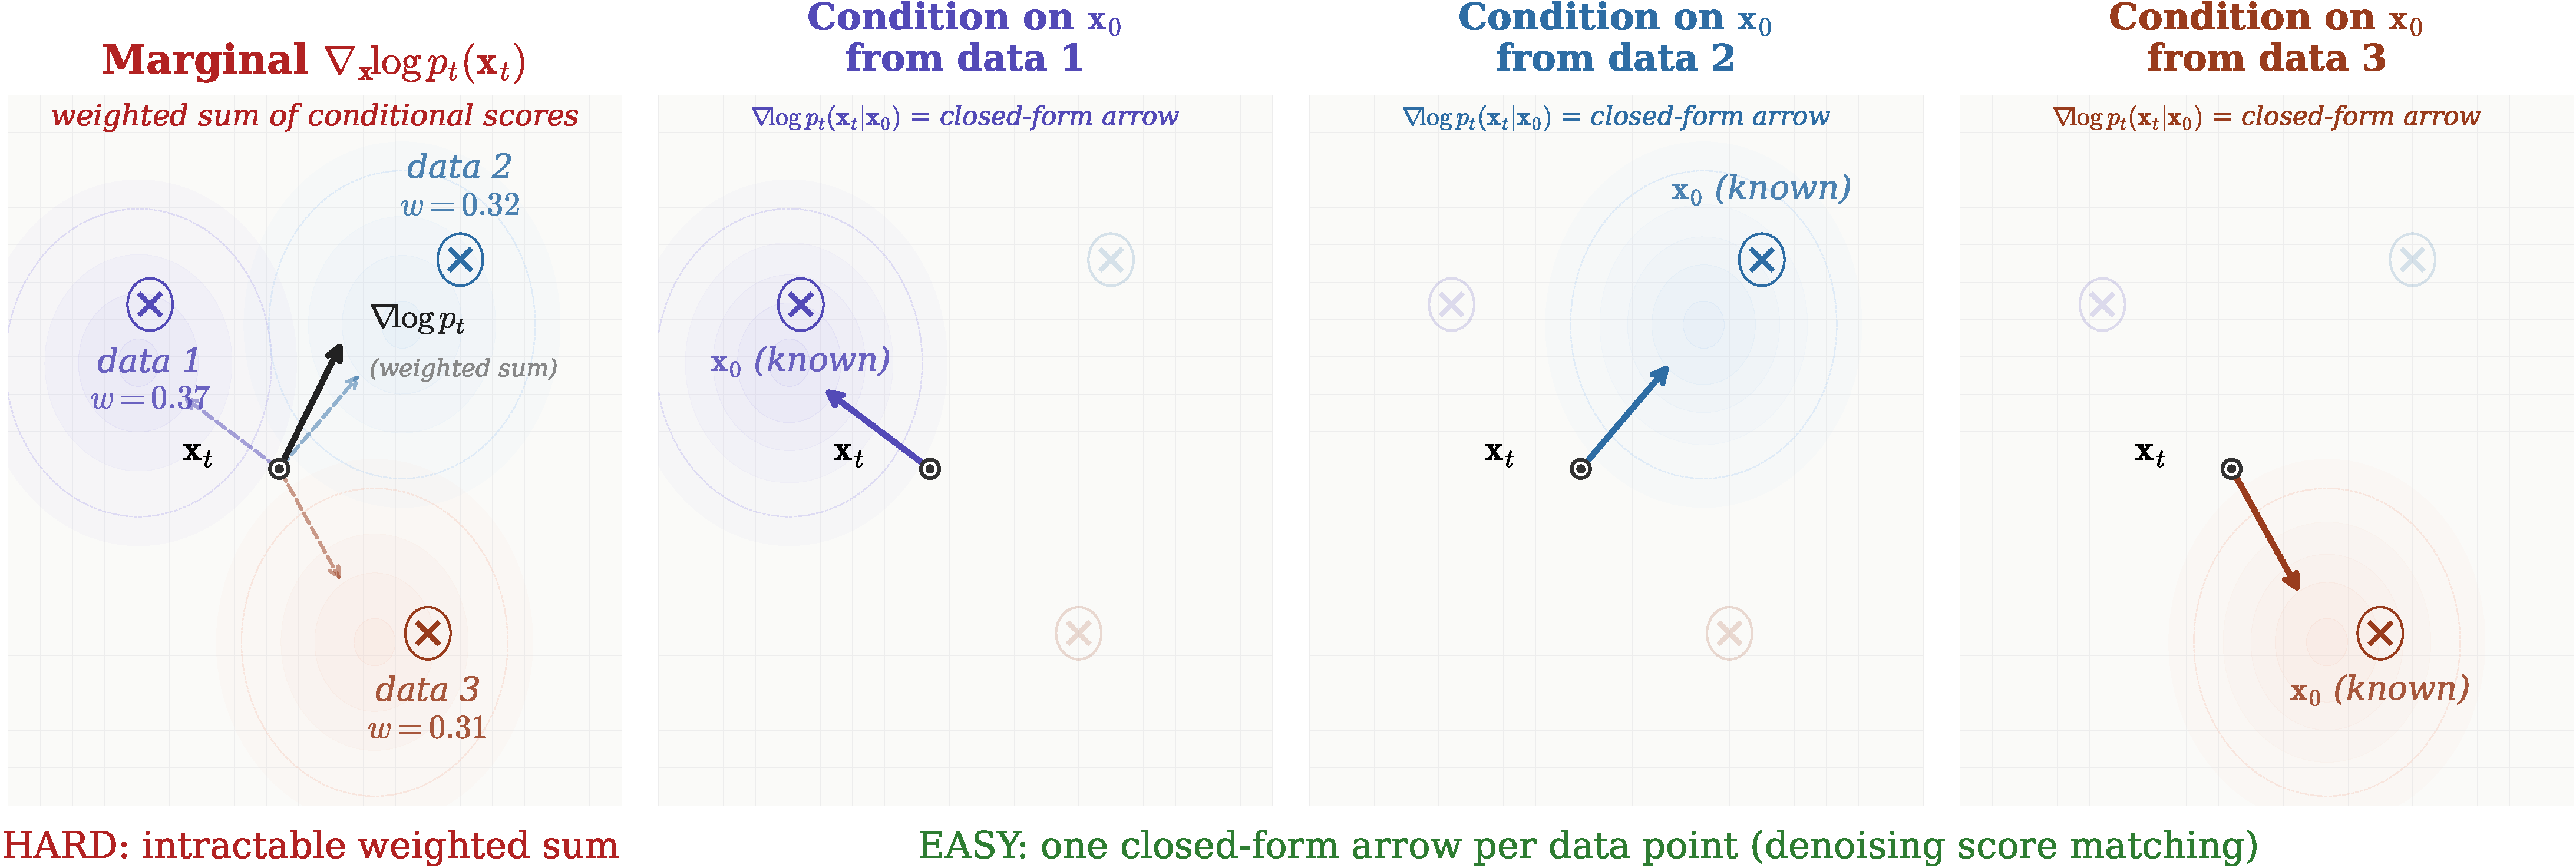
\includegraphics[width=\linewidth]{Images/PartB/denoising_score_matching.pdf}
    \caption{\textbfs{去噪分数匹配技巧的示意图。}
边缘分数 $\nabla_{\rvx_t}\log p_t(\rvx_t)$ 通常是所有可能的干净样本 $\rvx_0$ 上条件分数的难以处理的加权平均，其权重由在含噪观测 $\rvx_t$ 条件下 $\rvx_0$ 的后验分布给出。
然而，对于每个固定的 $\rvx_0$，条件分数 $\nabla_{\rvx_t}\log p_t(\rvx_t|\rvx_0)$ 具有闭式表达。
去噪分数匹配将这一困难的边缘估计问题转化为容易的逐样本回归问题。
\figcredit{由作者借助 AI 辅助编程绘制。}}
    \label{fig:score-and-denoising-score}
\end{figure}


为避免依赖难以处理的 oracle 分数 $\nabla_{\rvx} \log p_t(\rvx)$，我们采用 \Cref{eq:dsm-loss} 中的 DSM 损失。以数据点 $\rvx_0$ 为条件，该方法允许通过 \Cref{eq:score-gaussian-formula} 使用解析上易于处理的分数 $\nabla_{\rvx_t} \log p_t(\rvx_t|\rvx_0)$，具体例子见 \Cref{sec:instances}。具体而言，我们采用如下损失函数：
\begin{mdframed}
    \begin{equation}\label{eq:conti-dsm_loss-real}
\begin{aligned}
     &\mathcal{L}_{\text{DSM}}(\bm{\phi}; \omega(\cdot)) := \\
     &\frac{1}{2} \mathbb{E}_{t}  \mathbb{E}_{\rvx_0} \mathbb{E}_{ p_t(\rvx_t|\rvx_0)} \Big[\omega(t)\norm{\mathbf{s}_{\bm{\phi}}(\rvx_t, t) - \nabla_{\rvx_t} \log p_t(\rvx_t|\rvx_0)}_2^2 \Big],
\end{aligned}
\end{equation}
\end{mdframed}
其中 $\rvx_0 \sim p_{\mathrm{data}}$。\Cref{eq:conti-dsm_loss-real} 可以理解为 \Cref{eq:nscn} 的连续时间对应物，离散情形中的求和被积分替代。


类似定理~\ref{thm:sm-dsm} 中的结论，\Cref{eq:conti-dsm_loss-real} 的最小化子唯一确定如下：

\proppp{DSM 的最小化子}{dsm-minimizer}{
最小化子 $\mathbf{s}^*$ 满足
\begin{align}\label{eq:optimal-score}
\begin{aligned}
    \mathbf{s}^*(\rvx_t, t) 
    = \mathbb{E}_{\rvx_0 \sim p(\rvx_0 | \rvx_t)} \big[ \nabla_{\rvx_t} \log p_t(\rvx_t | \rvx_0) \big]= \nabla_{\rvx_t} \log p_t(\rvx_t),
\end{aligned}
\end{align}
对几乎所有的 $\rvx_t \sim p_t$ 与 $t \in [0,T]$ 成立。}{ 
DSM 目标可以理解为一个最小二乘误差问题。具体而言，在每个时刻 $t$，最优分数函数由对数条件密度梯度的条件期望给出，而根据贝叶斯法则，这等价于对数边缘密度的梯度。详细证明见附录~\ref{app-sec:min-dsm}。
}


\subsection{采样与推断}\label{subsec:sde-sample}
\begin{figure}[th!]
    \centering
    \vspace{-0.8cm}
    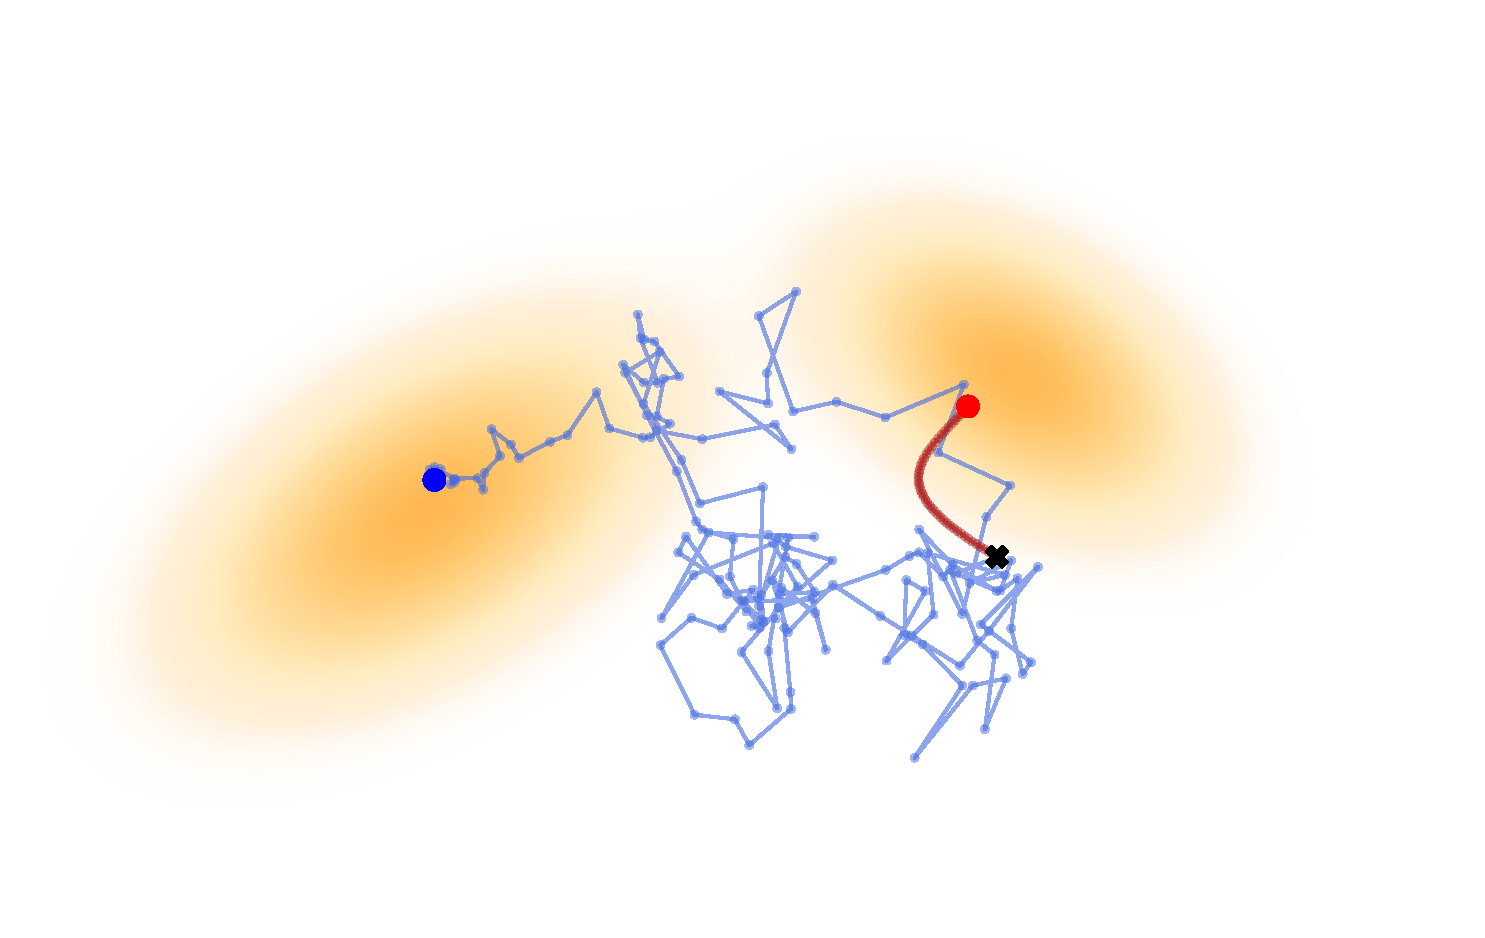
\includegraphics[width=\linewidth]{Images/PartB/sde_ode_trajectories.pdf}
    \vspace{-0.6cm}
    \caption{\textbfs{（二维）从 Score SDE 采样的示意图。}前向 SDE 设计为 $\diff\rvx(t)=\sqrt{2t}\diff\rvw(t)$，其漂移项 $\mathbf{f}\equiv\mathbf{0}$、扩散系数 $g(t)=\sqrt{2t}$（在 $[0,T]$ 上），将双峰高斯混合 $p_0=p_{\mathrm{data}}$ 演化为 $p_T\approx p_{\mathrm{prior}}:=\mathcal{N}(\mathbf{0},T^2\mathbf{I})$。图中展示了反向时间 SDE（蓝色；由 \Cref{eq:euler-maruyama} 求解）和 PF-ODE（红色；由 \Cref{eq:euler-ode} 求解）的采样轨迹。从随机点 $\rvx_T\sim p_{\mathrm{prior}}$（深色``$\times$''）出发，两条轨迹都随着 $t\to 0$ 朝 $p_{\mathrm{data}}$ 的支撑集移动。
    \figcredit{由作者绘制。}}
    \label{fig:sde_ode_trajectories}
\end{figure}


在学得
\[
\mathbf{s}_{\bm{\phi}^\times} := \mathbf{s}_{\bm{\phi}^\times}(\rvx, t) \approx \nabla_{\rvx} \log p_t(\rvx),
\]
之后，我们将反向时间 SDE（\Cref{eq:sde_backward}）与 PF-ODE（\Cref{eq:prob_ode_gt}）中难以处理的 oracle 分数 $\nabla_{\rvx} \log p_t(\rvx)$ 替换为学得的代理 $\mathbf{s}_{\bm{\phi}^\times}(\rvx, t)$。这一替换使得通过 SDE 或 ODE 进行易于处理的推断成为可能。为清楚起见，我们将所得过程分别记为 $\rvx^{\mathrm{SDE}}_{\bm{\phi}^\times}(t)$ 和 $\rvx^{\mathrm{ODE}}_{\bm{\phi}^\times}(t)$，但在后续章节中将省略这一区分。\footnote{这是为了在本小节之后简化记号。}

\paragraph{经验反向时间 SDE。}
通过在 \Cref{eq:sde_backward} 中用训练好的分数模型 $\mathbf{s}_{\bm{\phi}^\times}$ 替换真实分数，我们得到用于生成的参数化反向时间 SDE：
\begin{equation}\label{eq:sde_backward_sub}
    \diff \rvx^{\mathrm{SDE}}_{\bm{\phi}^\times}(t) = \left[\mathbf{f}\left(\rvx^{\mathrm{SDE}}_{\bm{\phi}^\times}(t), t\right) - g^2(t) \mathbf{s}_{\bm{\phi}^\times}\left(\rvx^{\mathrm{SDE}}_{\bm{\phi}^\times}(t), t\right) \right] \diff t + g(t) \diff \bar{\rvw}(t).
\end{equation}
为生成一个样本，我们首先从先验分布 $p_{\mathrm{prior}}$ 中抽取一个初始值 $\rvx_T$，然后从 $t=T$ 到 $t=0$ 反向数值求解 \Cref{eq:sde_backward_sub}。一种标准的数值求解器是 Euler–Maruyama 方法，它给出离散更新规则：
\begin{equation}\label{eq:euler-maruyama}
\rvx_{t - \Delta t} \leftarrow \rvx_t - \left[ \mathbf{f}(\rvx_t, t) - g^2(t)  \mathbf{s}_{\bm{\phi}^\times}(\rvx_t, t) \right] \Delta t + g(t) \sqrt{\Delta t} \cdot \boldsymbol{\epsilon},
\end{equation}
其中 $\boldsymbol{\epsilon} \sim \mathcal{N}(\bm{0}, \mathbf{I})$，$\Delta t > 0$ 为步长。

迭代这一更新规则即得到最终样本 $\rvx^{\mathrm{SDE}}_{\bm{\phi}^\times}(0)$。如果分数模型足够精确，这些生成样本的分布（记为 $p_{\bm{\phi}^\times}^{\mathrm{SDE}}(\cdot; 0)$）能很好地逼近真实数据分布\footnote{在理论上，估计精度取决于 $p_T$ 与 $p_{\mathrm{prior}}$ 之间的差异（通常可忽略）、模型训练误差以及数值离散化误差~\citep{de2022convergence,wang2024evaluating}。我们此处不追求形式化的界。}：
\[
p_{\bm{\phi}^\times}^{\mathrm{SDE}}(\cdot; 0) \approx p_{\mathrm{data}}(\cdot).
\]
事实上，\Cref{eq:ddpm-sampling} 中给出的 DDPM 采样方案正是这一 Euler–Maruyama 离散化在特定 $\mathbf{f}$ 和 $g$ 选择下的特例（见 \Cref{sec:instances}）。


\paragraph{经验 PF-ODE。}
PF-ODE 定义了一条连接 $p_{\mathrm{prior}}$ 与 $p_{\mathrm{data}}$ 的连续流，使得采样、编码以及精确的似然计算成为可能。下文针对每一种操作提供了进一步细节。
\subparagraph{I. 使用 PF-ODE 采样。}将 \Cref{eq:prob_ode_gt} 中的 oracle 分数替换为 $\mathbf{s}_{\bm{\phi}^\times}$，得到经验 PF-ODE：
\begin{equation}\label{eq:prob_ode_sub}
    \frac{\diff}{\diff t} \rvx^{\mathrm{ODE}}_{\bm{\phi}^\times}(t) = \mathbf{f}\left(\rvx^{\mathrm{ODE}}_{\bm{\phi}^\times}(t), t\right) - \frac{1}{2} g^2(t) \mathbf{s}_{\bm{\phi}^\times}\left(\rvx^{\mathrm{ODE}}_{\bm{\phi}^\times}(t), t\right).
\end{equation}
为生成样本，我们首先从先验分布 $p_{\mathrm{prior}}$ 中抽取一个初始样本 $\rvx_T$。然后从 $t=T$ 到 $t=0$ 反向数值求解 \Cref{eq:prob_ode_sub} 中的 PF-ODE。这一过程等价于逼近如下积分：
\[
\rvx^{\mathrm{ODE}}_{\bm{\phi}^\times}(0) = \rvx_T + \int_T^0 \left[ \mathbf{f}\left(\rvx^{\mathrm{ODE}}_{\bm{\phi}^\times}(\tau), \tau\right) - \frac{1}{2} g^2(\tau) \mathbf{s}_{\bm{\phi}^\times}\left(\rvx^{\mathrm{ODE}}_{\bm{\phi}^\times}(\tau), \tau\right) \right] \mathrm{d}\tau.
\]
求解这一积分得到最终样本 $\rvx^{\mathrm{ODE}}_{\bm{\phi}^\times}(0)$。通过这一确定性过程生成的样本分布（记为 $p_{\bm{\phi}^\times}^{\mathrm{ODE}}(\cdot; 0)$）给出了对数据分布的逼近，即 $p_{\bm{\phi}^\times}^{\mathrm{ODE}}(\cdot; 0) \approx p_{\mathrm{data}}$。

设 $\Delta t > 0$ 为离散化步长。一种标准的数值积分方法是 Euler 方法，它估计
\[
\mathbf{f}(\rvx_\tau, \tau) - \frac{1}{2} g^2(\tau)  
\mathbf{s}_{\bm{\phi}^\times}(\rvx_\tau, \tau) \approx \mathbf{f}(\rvx_t, t) - \frac{1}{2} g^2(t)  
\mathbf{s}_{\bm{\phi}^\times}(\rvx_t, t), \quad \tau \in [t-\Delta t, t],
\]
得到如下更新规则：
\begin{equation}\label{eq:euler-ode}
\rvx_{t - \Delta t} \leftarrow \rvx_t -
\left[ \mathbf{f}(\rvx_t, t) - \frac{1}{2} g^2(t)  
\mathbf{s}_{\bm{\phi}^\times}(\rvx_t, t) \right] \Delta t.
\end{equation}


这一联系使我们能够用如下核心洞见重新表述生成过程：
\msg{洞见}{生成 $\Leftrightarrow$ 求解 ODE/SDE}{从扩散模型采样在根本上等价于求解相应的概率流 ODE 或反向时间 SDE。}

这一等价性清晰地解释了扩散模型采样速度慢的问题，正如问题~\ref{ques:dm-sampling-slow} 所提出的。生成之所以计算密集，是因为这些微分方程的数值求解器本质上是迭代的，通常需要许多步才能准确逼近一条解轨迹\footnote{例如，DDPM 与 Score SDE 通常使用 $1{,}000$ 次函数计算来完成生成。}。然而，PF-ODE 的表述也是有利的，因为它使我们能够利用关于加速数值求解器的丰富文献。探索这些技术以加速扩散模型采样是 \Cref{ch:solvers} 的主要焦点。



\subparagraph{II. 使用 PF-ODE 的反演。}如前所述，与 SDE 的情形不同，我们可以沿正向（从 $0$ 到 $T$）与反向（从 $T$ 到 $0$）两个方向求解同一个 \Cref{eq:prob_ode_sub}。当沿正向求解时，ODE 流将数据映射为它在所有 $t \in [0,T]$ 处的（含噪）隐表示，扮演了编码器的角色。这一概念为可控生成（如图像翻译与编辑等）带来了强大的应用~\citep{mokady2023null,su2022dual}。

\subparagraph{III. 通过 PF-ODE 进行精确对数似然计算。}
我们将 \Cref{eq:prob_ode_sub} 中的动力学重新解释为神经 ODE~\citep{chen2018neural} 的一个变体（在 \Cref{subsec:NODE} 中介绍），它仅参数化分数函数，而非完整的速度场。这一 PF-ODE 表述通过变量替换公式实现了精确的对数似然计算。

将 \Cref{eq:instant-change-of-var} 中的恒等式应用于 \Cref{eq:prob_ode_sub} 中的 PF-ODE，我们定义速度场为
\[
\rvv_{{\bm{\phi}^\times}}(\rvx, t) := \rvf(\rvx, t) - \frac{1}{2}g^2(t)\rvs_{\bm{\phi}^\times}(\rvx, t),
\]
其中使用了学得的分数 $\rvs_{\bm{\phi}^\times}$。沿 PF-ODE 轨迹 $\{\rvx^{\mathrm{ODE}}_{\bm{\phi}^\times}(t)\}_{t \in [0, T]}$，对数密度 $p^{\textup{ODE}}_{\bm{\phi}^\times}(\cdot; t)$ 的时间演化满足
\begin{align*}
    \frac{\diff}{\diff t} \log p^{\textup{ODE}}_{\bm{\phi}^\times}\big(\rvx^{\mathrm{ODE}}_{\bm{\phi}^\times}(t), t \big) 
    &= -\nabla \cdot \rvv_{{\bm{\phi}^\times}}\left(\rvx^{\mathrm{ODE}}_{\bm{\phi}^\times}(t), t  \right),
\end{align*}
其中 $\nabla \cdot \mathbf{v}$ 表示在 $\rvx$ 上的散度。

为评估一个数据点 $\rvx_0 \sim p_{\mathrm{data}}$ 的似然，我们从 $t=0$ 到 $t=T$ 积分如下的增广 ODE 系统：
\begin{align}\label{eq:score-sde-likelihood}
\frac{\diff}{\diff t}
\begin{bmatrix}
\mathbf{x}(t) \\
\delta(t)
\end{bmatrix}
=
\begin{bmatrix}
\rvv_{{\bm{\phi}^\times}}(\mathbf{x}(t), t) \\
-\nabla \cdot \rvv_{{\bm{\phi}^\times}}(\mathbf{x}(t), t)
\end{bmatrix}, \quad
\begin{bmatrix}
\mathbf{x}(0) \\
\delta(0)
\end{bmatrix}
=
\begin{bmatrix}
\mathbf{x}_0 \\
0
\end{bmatrix},
\end{align}
其中 $\delta(t)$ 累积随时间变化的对数密度变化。将系统求解至 $t = T$ 后，我们得到终止状态：
\[
\begin{bmatrix}
\rvx(T) \\
\delta(T)
\end{bmatrix}.
\]
于是，原始样本 $\rvx_0$ 在模型下的对数似然可计算为
\[
\log p^{\textup{ODE}}_{\bm{\phi}^\times}(\rvx_0; 0) = \log p_{\mathrm{prior}}\left( \rvx(T) \right) + \delta(T),
\]
其中 $ p_{\mathrm{prior}}\left(\rvx(T)\right) $ 表示在 $ \rvx(T) $ 处取值的闭式先验密度。

% \se{should cite the neural ode paper}



\newpage

\section{SDE 的实例化}\label{sec:instances}

\citet{song2020score} 根据演化过程中方差的行为，将前向 SDE 中的漂移项 $\rvf(\rvx, t)$ 和扩散项 $g(t)$ 分为三类。这里我们关注两种常用类型：\emph{\underline{V}ariance \underline{E}xplosion}（爆方差，VE）SDE 和 \emph{\underline{V}ariance \underline{P}reserving}（保方差，VP）SDE。虽然可以设计自定义的噪声调度，但其设计会显著影响经验表现。
表~\ref{tb:sde_instances} 总结了这两种 SDE 实例化。
\begin{table}[th]
  \caption{前向 SDE 总结}
  \small
  \centering
  \resizebox{\textwidth}{!}{
  \begin{tabular}{cccc}
     \toprule
    
         &   \textbfs{VE SDE}   & \textbfs{VP SDE}  \\
       \midrule
    $\mathbf{f}(\rvx, t)$ & $\mathbf{0} $   &  $-\frac{1}{2}\beta(t)\rvx$  \\
      $g(t)$   & $\sqrt{\frac{\diff \sigma^2(t)}{\diff t}}$ 
      % $\sigma_{\textup{min}}\Big(\frac{\sigma_{\textup{max}}}{\sigma_{\textup{min}}} \Big)^t\sqrt{2\log \big(\frac{\sigma_{\textup{max}}}{\sigma_{\textup{min}}}\big)}$
       &  $\sqrt{\beta(t)}$  \\

    SDE   &   $\diff\rvx(t) =  g(t) \diff\rvw(t)$    &   $\diff\rvx(t) = -\frac{1}{2}\beta(t) \rvx(t) \diff t + \sqrt{\beta(t)} \diff\rvw(t)$ \\
   \midrule
     $p_t(\rvx_t|\rvx_0)$   & $        \mathcal{N}\left(\rvx_t ; \rvx_0, \left(\sigma^2(t) - \sigma^2(0)\right)\rmI\right)$     &  $ \mathcal{N}\left(\rvx_t ; \rvx_0 e^{-\frac{1}{2}\int_{0}^{t} \beta(\tau)\diff \tau}, \rmI - \rmI e^{-\int_{0}^{t} \beta(\tau)\diff \tau}\right)$ \\
   
     $p_{\mathrm{prior}}$   & $ \mathcal{N}(\bm{0}, \sigma^2(T)\rmI)$    &  $\mathcal{N}(\bm{0}, \rmI)$  \\
 \bottomrule
  \end{tabular}
  }
  \label{tb:sde_instances}
\end{table}




\subsection{VE SDE}
VE SDE 具有如下组成部分：
\begin{itemize}
    \item \textbfs{漂移项：}零漂移项 $\mathbf{f}=\bm{0}$。
    \item \textbfs{扩散项：}$g(t)=\sqrt{\frac{\diff \sigma^2(t)}{\diff t}}$，其中 $\sigma(t)$ 为某个函数。
\end{itemize}
前向 SDE 取如下形式：
\begin{equation}\label{eq:vesde}
    \diff\rvx(t) =  \sqrt{\frac{\diff \sigma^2(t)}{\diff t}} \diff\rvw(t).
\end{equation} 
类似地，\Cref{subsec:scoresde-perturbation-kernel} 的结果蕴含了 VE SDE 的扰动核，并建议选择合适的先验分布：
\begin{itemize}
    \item \textbfs{扰动核：}
\begin{align*}
        p_t(\rvx_t | \rvx_0) &= \mathcal{N}\left(\rvx_t ; \rvx_0, \left(\sigma^2(t) - \sigma^2(0)\right)\rmI\right) 
\end{align*}
    \item \textbfs{先验分布：}假设 $\sigma(t)$ 在 $t \in [0,T]$ 上是递增函数，且 $\sigma^2(T) \gg \sigma^2(0)$。先验分布为：
    \[
    p_{\mathrm{prior}} := \mathcal{N}(\bm{0}, \sigma^2(T)\rmI).
    \]
\end{itemize}

VE SDE 的一个典型实例是 NCSN，其设计如下：
\[
\sigma(t):=\sigma_{\textup{min}}\left(\frac{\sigma_{\textup{max}}}{\sigma_{\textup{min}}} \right)^t,\quad \text{for } t\in(0,1],
\]
其中 $\sigma_{\textup{min}}$ 和 $\sigma_{\textup{max}}$ 是预先指定的常数。也就是说，方差序列被设计为几何序列。由此，NCSN 可被视为 VE SDE 的离散化版本，正如 \Cref{subsec:scoresde-motivation} 中所讨论的。

% \paragraph{(Optional) Brief Introduction to EDM~\citep{karras2022elucidating}.}
% \citet{karras2022elucidating} study a special class of VE-type SDEs with carefully designed neural network parametrizations, time schedules, noise schedulers, weighting functions, and ODE samplers. They focus on the following PF-ODE, where time $t$ is reparametrized as variance $\sigma(t)$:
% \[
%     \diff \rvx(t) = - \sigma'(t) \sigma(t) \nabla_{\rvx} \log p(\rvx, \sigma(t)) \diff t.
% \]
% A common choice for the diffusion coefficient is
% \begin{itemize}
%     \item \textbfs{Diffusion term:} $\sigma(t) = t$, or equivalently, 
%     \[
%     g(t) = \sqrt{\frac{\diff \sigma^2(t)}{\diff t}} = \sqrt{2t}.
%     \]
% \end{itemize}
% This yields the forward SDE and corresponding PF-ODE:
% \begin{align*}
%     \diff \rvx(t) &= \sqrt{2t}   \diff \rvw(t), \\
%     \diff \rvx(t) &= - t   \nabla_{\rvx} \log p_t(\rvx(t))   \diff t.
% \end{align*}
% The associated perturbation kernel and prior distribution are given by:
% \begin{itemize}
%     \item \textbfs{Perturbation kernel:}
%     \[
%         p_t(\rvx_t | \rvx_0) = \mathcal{N}(\rvx_t; \rvx_0, t^2 \mathbf{I}),
%     \]
%     \item \textbfs{Prior distribution:}
%     \[
%         p_{\mathrm{prior}} = \mathcal{N}(\mathbf{0}, T^2 \mathbf{I}).
%     \]
% \end{itemize}
% Further discussion on EDM is provided in \Cref{subsec:D-design-edm}.



\subsection{VP SDE}
设 $\beta\colon [0,T] \rightarrow \mathbb{R}_{\geq 0 }$ 为关于 $t$ 的非负函数。VP SDE 由如下组成部分定义：
\begin{itemize}
    \item \textbfs{漂移项：}线性漂移 $\mathbf{f}(\rvx, t) = -\frac{1}{2}\beta(t)\rvx$。
    \item \textbfs{扩散项：}$g(t) = \sqrt{\beta(t)}$。
\end{itemize}
于是前向 SDE 表达为：
\begin{align}\label{eq:forward-linear-sde}
\diff\rvx(t) = -\frac{1}{2}\beta(t) \rvx(t) \diff t + \sqrt{\beta(t)} \diff\rvw(t).
\end{align}

利用 \Cref{subsec:scoresde-perturbation-kernel} 的结果，我们可以推导 VP SDE 的扰动核并选择合适的先验分布：
\begin{itemize}
    \item \textbfs{扰动核：}
    \[
    p_t(\rvx_t|\rvx_0) = \mathcal{N}\left(\rvx_t ; \rvx_0 e^{-\frac{1}{2}\int_{0}^{t} \beta(\tau)\diff \tau}, \rmI - \rmI e^{-\int_{0}^{t} \beta(\tau)\diff \tau}\right).
    \]
    \item \textbfs{先验分布：}$p_{\mathrm{prior}} := \mathcal{N}(\bm{0}, \rmI)$。
\end{itemize}
我们指出，由于扰动核是具有已知均值和协方差的高斯，我们可以应用 \Cref{eq:gaussian-score} 来计算其分数函数。

VP SDE 的一个经典例子是 DDPM，其噪声调度 $\beta(t)$ 定义为：
\[
\beta(t) := \beta_{\textup{min}} + t(\beta_{\textup{max}} - \beta_{\textup{min}}), \quad \text{for all } t \in [0,1].
\]
这里 $\beta_{\textup{min}}$ 和 $\beta_{\textup{max}}$ 是预定义的常数。由此，DDPM 可被解释为 VP SDE 的离散化，正如 \Cref{subsec:scoresde-motivation} 中所讨论的.




\subsection{（选读）扰动核 $ p_t(\rvx_t|\rvx_0) $ 是如何推导的？}\label{subsec:scoresde-perturbation-kernel}
如果前向 SDE（\Cref{eq:sde_forward}）中的漂移项关于 $\rvx$ 是线性的，取如下形式
\begin{align*}
    \rvf(\rvx, t) = f(t) \rvx,
\end{align*}
其中 $f(t) \in \mathbb{R}$ 是某个标量值、时间依赖的函数，那么 \Cref{eq:sde_forward} 就成为一个线性 SDE：
\[
\diff\rvx(t) = f(t)\rvx(t) \diff t + g(t) \diff\rvw(t).
\]


即使初始分布 $p_{\mathrm{data}}$ 是非高斯的，漂移项的线性也确保条件过程保持高斯性。特别地，对 $t>0$，转移核具有如下形式：
\[
p_t( \rvx_t | \rvx_0 ) = \mathcal{N} \left( \rvx_t;  \rvm(t),  P(t) \mathbf{I}_D \right),
\]
其中 $\rvx_0 \sim p_{\mathrm{data}}$，$\rvm(t) \in \mathbb{R}^D$，$P(t)\in\mathbb{R}_{\ge 0}$ 分别表示给定 $\rvx_0$ 时的条件均值与（标量）方差，定义为：
\[
\rvm(t) = \mathbb{E} \left[\rvx_t | \rvx(0) = \rvx_0\right], \qquad
P(t) \mathbf{I}_D = \operatorname{Cov} \left[\rvx_t | \rvx(0) = \rvx_0\right].
\]

这一阶矩与二阶矩按如下 ODE 演化~\citep{sarkka2019applied}：
\begin{align}\label{eq:mean-var-evolution}
\begin{aligned}
    \frac{\diff \rvm(t)}{\diff t} &= f(t) \rvm(t), \\
    \frac{\diff P(t)}{\diff t} &= 2f(t) P(t) + g^2(t),
\end{aligned}
\end{align}
只要初始均值 $\rvm(0)$ 与方差 $P(0)$ 有限即可。

由于这两个 ODE 都是线性的，它们可通过积分因子法求得闭式解。
给定初始条件 $\rvx_0$，均值与方差演化为
\begin{align}\label{eq:mean-var-solution}
    \rvm(t) = \mathcal{E}(0  \to  t) \rvx_0, 
\qquad 
P(t) = \int_{0}^{t} \mathcal{E}^{2}(s  \to  t)  g(s)^{2} \diff s,
\end{align}
其中 $\rvm(0)=\rvx_0$，$P(0)=0$。
这里 $\mathcal{E}(s  \to  t)$ 表示指数积分因子
\[
\mathcal{E}(s  \to  t) := \exp \left(\int_{s}^{t} f(u) \diff u\right),
\]
它刻画了漂移项从时刻 $s$ 到 $t$ 的累积效应。因此，转移核 $p_t(\rvx_t | \rvx_0)$ 也具有闭式表达。

我们将如下论断的证明推迟到 \Cref{subsec:rigorous-proof-linear-sde}：即在坐标独立、扩散系数为 $g(t)\mathbf I_D$ 的 $D$ 维 Wiener 过程下 $p_t(\rvx_t |\rvx_0)$ 的条件协方差是各向同性的，即 
$\operatorname{Cov}[\rvx_t | \rvx_0] = P(t) \mathbf I_D$，以及 \Cref{eq:mean-var-evolution} 的推导，它们依赖于 Itô 微积分。


\exm{VE SDE 的转移核}{在 VE SDE 的特殊情形下：$\rvf \equiv 0$ 且 $g(t) = \sqrt{\frac{\diff \sigma^2(t)}{\diff t}}$，SDE 解的均值与协方差按如下方式演化。

\proofparagraph{均值。}
\[
\frac{\diff \rvm(t)}{\diff t} = 0, 
\quad \text{with} \quad \rvm(0) = \rvx_0
 \Longrightarrow 
\rvm(t) = \rvx_0.
\]

\proofparagraph{方差。}
\[
\frac{\diff P(t)}{\diff t} = \frac{\diff \sigma^2(t)}{\diff t},
\quad \text{with} \quad P(0) = 0
 \Longrightarrow 
P(t) = \sigma^2(t) - \sigma^2(0).
\]
因此
\[
p_t(\rvx_t | \rvx_0)=\mathcal{N} \left(\rvx_t;  \rvx_0,  \big(\sigma^2(t)-\sigma^2(0)\big)\mathbf{I}_D\right).
\]
}

\exm{VP SDE 的转移核}{在 VP SDE 的情形下，漂移项为 $\rvf(\rvx, t) = -\tfrac{1}{2}\beta(t) \rvx$，扩散项为 $g(t) = \sqrt{\beta(t)}$：

\proofparagraph{均值 $\rvm(t)$。}
\[
\frac{\diff \rvm}{\diff t}
= -\frac{1}{2}\beta(t) \rvm(t),
\quad
B(t) \coloneqq \int_{0}^{t} \beta(s) \diff s,
\quad
\rvm(t) = e^{-\frac{1}{2}B(t)} \rvx_0.
\]

\proofparagraph{方差 $P(t)$。} 方差满足
\[
\frac{\diff P}{\diff t} = -\beta(t) P(t) + \beta(t).
\]
应用积分因子 $e^{B(t)}$（其中 $B(t) = \int_0^t \beta(s) \diff s$），得到
\[
\frac{\diff}{\diff t} \left[P(t)e^{B(t)}\right] = \beta(t) e^{B(t)}.
\]
两边积分得
\[
P(t) = 1 - e^{-B(t)}.
\]
因此协方差是各向同性的，且
\[
\rmP(t) = P(t) \mathbf I_D = \bigl(1 - e^{-B(t)}\bigr)\mathbf I_D.
\]

\proofparagraph{最终闭式转移核。}
\[
p_t(\rvx_t\mid\rvx_0)
= \mathcal{N} \left(
   \rvx_t; 
   \underbrace{e^{-\frac{1}{2} B(t)} \rvx_0}_{\rvm(t)}, 
   \underbrace{\big(1 - e^{-B(t)}\big)\mathbf{I}_D}_{P(t)\mathbf{I}_D}
\right),
\quad
B(t) = \int_0^t \beta(s) \diff s.
\]
}

\clearpage
\newpage


\section{\texorpdfstring{重新审视分数基与变分扩散模型中的前向核}{Rethinking Forward Kernels in Score-Based and Variational Diffusion Models}}\label{sec:variational-perspective}

% \se{do we need this section? feels a bit pedantic, not necessarily getting at the core idea}

DDPM 与 Score SDE 通常是通过前向转移核 $ p(\rvx_t|\rvx_{t-\Delta t}) $ 引入的，在 DDPM 中以离散方式定义，而在 Score SDE 中以连续时间 SDE 定义。然而，实际中最相关的——尤其在它们的损失函数（\Cref{eq:ddpm-mean-loss,eq:conti-dsm_loss-real}）中——是从数据出发的累积转移核 $ p_t(\rvx_t|\rvx_0) $。两个框架最终都依赖于这个核，要么通过递归计算（DDPM），要么通过求解一个 ODE（见 \Cref{subsec:scoresde-perturbation-kernel}，Score SDE）。

在本节中，我们从定义 $ p_t(\rvx_t|\rvx_0) $（在连续时间下）开始，它提供了一个更整洁、更直接的视角。总体而言，尽管 $ p(\rvx_t|\rvx_{t-\Delta t}) $ 与 $ p_t(\rvx_t|\rvx_0) $ 在理论上是等价的，但定义后者往往得到更干净、更具可解释性的表述。特别地，$ p_t(\rvx_t|\rvx_0) $ 在 $ t \to T $ 时对先验提供了直接的洞察，并与实际的损失设计自然契合。
\begin{figure}[th!]
    \centering
    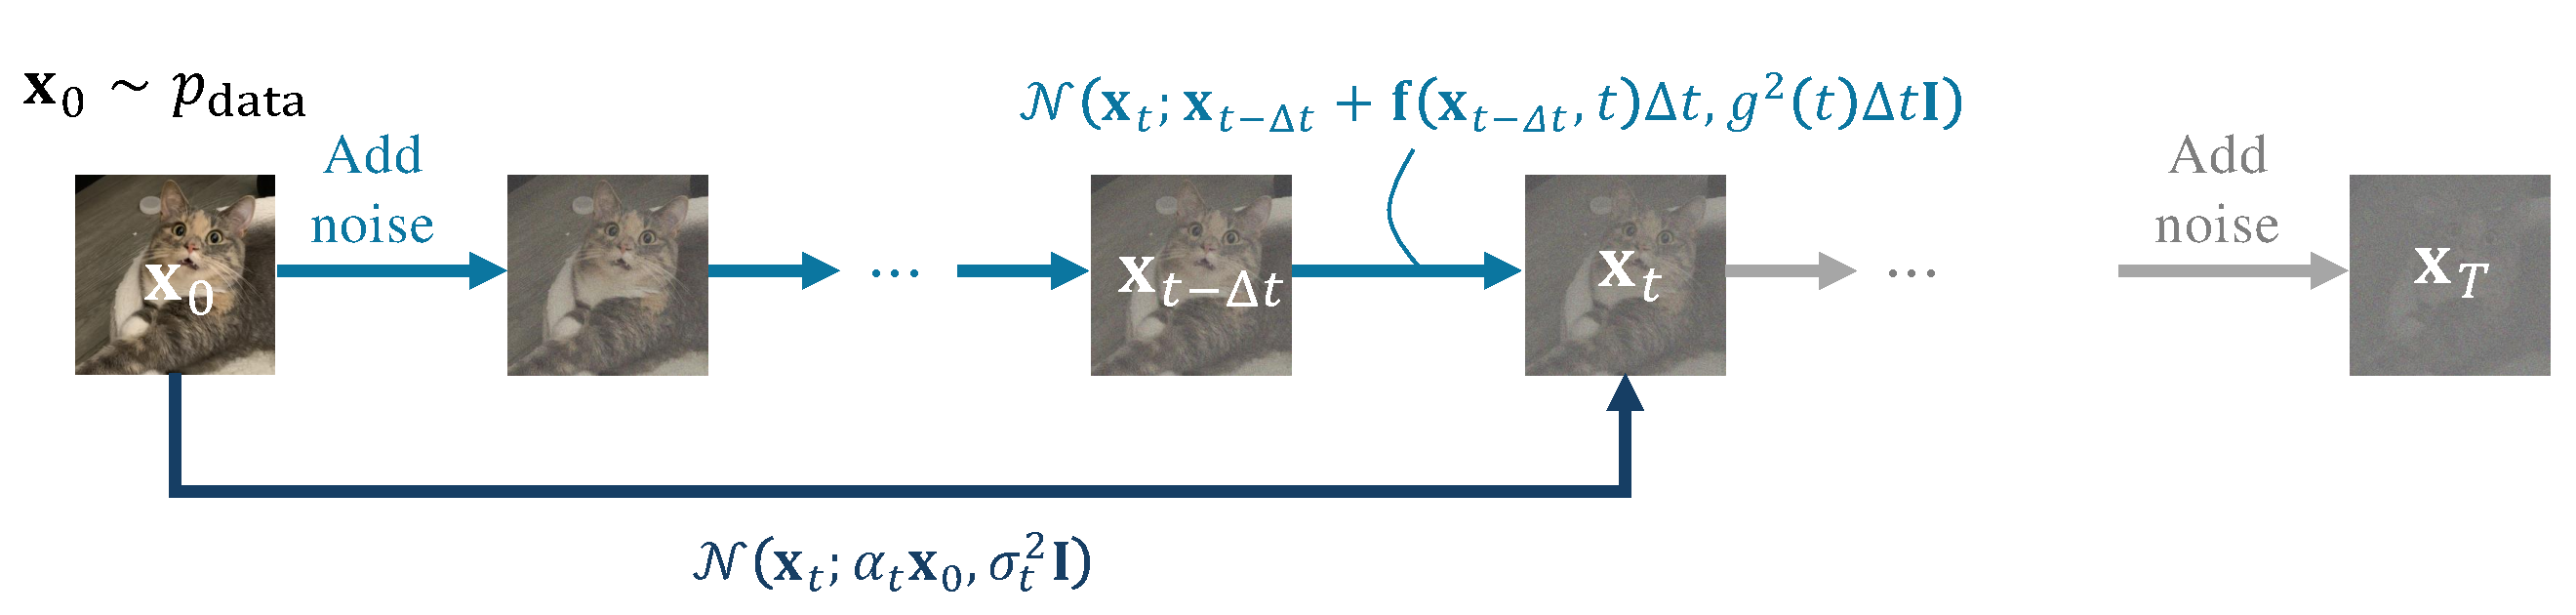
\includegraphics[width=\linewidth]{Images/PartB/vdm-sde.pdf}
    \caption{\textbfs{引理~\ref{forward-sde} 的示意图。}通过连续时间 SDE（$\Delta t\to 0$）的增量噪声注入与 \Cref{eq:forward_kernel} 的直接扰动在数学上等价。 \figcredit{由作者绘制。}}
    \label{fig:vdm-sde}
\end{figure}
\subsection{一般的仿射前向过程 $p_t(\rvx_t |\rvx_0)$}
我们先定义一个一般的前向扰动核：
\begin{equation}\label{eq:forward_kernel}
p_t(\rvx_t| \rvx_0) := \mathcal{N}\big(\rvx_t; \alpha_t \rvx_0, \sigma_t^2 \mathbf{I}\big),
\end{equation}
其中 $\rvx_0 \sim p_{\mathrm{data}}$，$\alpha_t$、$\sigma_t$ 是 $t \in [0,T]$ 的非负标量函数，满足：
\begin{enumerate}
    \item[(i)] 对所有 $t \in (0,1]$，$\alpha_t > 0$ 且 $\sigma_t > 0$（允许 $\sigma_0 = 0$），且
    \item[(ii)] 通常 $\alpha_0 = 1$ 且 $\sigma_0 = 0$。
\end{enumerate}
也就是说，$\rvx_t \sim p_t(\rvx_t | \rvx_0)$ 可以采样为
\begin{equation*}
\rvx_t = \alpha_t \rvx_0 + \sigma_t \bm{\epsilon}, 
\qquad \bm{\epsilon} \sim \mathcal{N}(\mathbf{0}, \mathbf{I}).
\end{equation*}

这一框架涵盖了若干著名的实例，包括 VE（例如 NCSN）、VP（例如 DDPM）以及流匹配（FM）前向核~\citep{lipman2022flow, liu2022rectified}，后者在 $\rvx_0$ 和 $\bm{\epsilon}$ 之间做线性插值（见后文 \Cref{sec:flow-matching-framework}）。
\begin{itemize}
\item \textbfs{VE（NCSN）核：}$\alpha_t \equiv 1$，$\sigma_T \gg 1$；
\item \textbfs{VP（DDPM）核：}$\alpha_t := \sqrt{1 - \sigma_t^2}$，使得 $\alpha_t^2 + \sigma_t^2 = 1$；
\item \textbfs{FM 核：}$\alpha_t = 1 - t$，$\sigma_t = t$。
\end{itemize}

\subsection{与 Score SDE 的联系}
对 Score SDE 而言，以线性形式指定 $ p_t(\rvx_t|\rvx_0) $ 自然地诱导出一个具有仿射系数的 SDE，这提供了比从漂移项和扩散项出发、为各矩求解 ODE（见 \Cref{subsec:scoresde-perturbation-kernel}）更直观的替代方案。

给定 \Cref{eq:forward_kernel} 中的前向扰动核，相应的前向 SDE 取如 \Cref{eq:forward-linear-sde} 的关于 $\rvx$ 线性的形式：
\begin{align*}
    \diff \rvx(t) = \underbrace{f(t)\rvx(t)}_{\rvf(\rvx(t), t)} \diff t + g(t) \diff\rvw(t),
\end{align*}
其中 $ f, g\colon [0,T] \rightarrow \mathbb{R} $ 是时间的实值函数。
系数 $ f(t) $ 和 $ g(t) $ 可以用 $ \alpha_t $ 和 $ \sigma_t $ 解析地表达，如下面的引理所总结。

\lemp{前向扰动核 $\Leftrightarrow$ 线性 SDE}{forward-sde}{ 对 $t\in(0,T]$ 定义 $\lambda_t:=\log\tfrac{\alpha_t}{\sigma_t}$。
给定前向扰动核
\[
\rvx_t=\alpha_t \rvx_0+\sigma_t \beps,\qquad \beps\sim\mathcal N(\mathbf 0,\rmI),
\]
线性 SDE
\[
\diff \rvx(t)=f(t) \rvx(t) \diff t+g(t) \diff\rvw(t),
\]
其系数为
\begin{align}\label{eq:kernel-sde-equiv}
\begin{aligned}
f(t)&=\frac{\diff}{\diff t}\log \alpha_t,\\
g^2(t)&=\frac{\diff \sigma_t^2}{\diff t}-2\frac{\diff}{\diff t}\log\alpha_t \sigma_t^2
       = -2\sigma_t^2 \frac{\diff}{\diff t}\lambda_t,
\end{aligned}
\end{align}
对所有 $t\in(0,T]$ 具有条件转移 $p_t(\rvx_t|\rvx_0)=\mathcal N \big(\rvx_t;\alpha_t\rvx_0,\sigma_t^2\rmI\big)$。
反之，若一个线性 SDE 的条件转移为 $\mathcal N(\rvx_t;\alpha_t\rvx_0,\sigma_t^2\rmI)$，使得对所有 $t\in(0,T]$ 都有 $\alpha_t>0$ 且 $\sigma_t>0$，则其系数对 $t\in(0,T]$ 满足 \Cref{eq:kernel-sde-equiv}。
}{由 \Cref{subsec:scoresde-perturbation-kernel}，证明就是将均值与协方差 ODE $\rvm'(t) = f(t)\rvm(t)$、$\rmP'(t) = 2f(t) \rmP(t) + g^2(t) \rmI$ 与
$\rvm(t)=\alpha_t\rvx_0$ 和 $\rmP(t)=\sigma_t^2\rmI$（在 $(0,T]$ 上）相匹配。}


\rmkb{要在终止时刻精确匹配一个高斯先验，过程必须完全遗忘 $\rvx_0$ 并达到目标方差；这要求 $\alpha_T=0$ 且 $\sigma_T^2$ 等于先验方差。

在 SDE 表述中，有
\[
\alpha_t=\exp \Big(\int_0^t f(u)\diff  u\Big).
\]
因此，在有限 $T$ 处强制 $\alpha_T=0$ 会迫使
\[
\int_0^T f(u)\diff u=-\infty,
\]
意味着漂移项必须随 $t\rightarrow T$ 无限快地收缩。
同时，扩散必须发散以维持所规定的方差，这反映在
\[
g^2(t)=\sigma_t^{2 \prime}-2\frac{\alpha_t'}{\alpha_t} \sigma_t^2  \rightarrow  \infty
\quad\text{as } t\rightarrow T.
\]

如果 $f$ 和 $g$ 在 $[0,T]$ 上保持有界，则必然有 $\alpha_T>0$ 且仍残留对 $\rvx_0$ 的依赖。此时，高斯先验只能渐近地达到：要么在 $t\to T$ 的极限下（但不能精确达到），要么在适当的时间重参数化后于 $T\to\infty$ 的无穷区间上精确达到。
}


由上述引理，通过具有系数 $f(t)$ 和 $g(t)$ 的线性 SDE 指定增量噪声注入，在数学上等价于以参数 $\alpha_t$ 和 $\sigma_t$ 定义扰动核。在扩散模型文献中，这两种视角可互换使用。因此，我们得出结论：
\msg{观察}{}{
定义 $p_t(\rvx_t | \rvx_0)$ 等价于指定线性 SDE 的系数 $f(t)$ 和 $g(t)$。
}


\subsection{与基于变分的扩散模型的联系}\label{subsec:connection-vdm}
我们重新审视 DDPM 中一个通过贝叶斯法则推导的核心恒等式：
\begin{align}\label{eq:ddpm-reverse-condition-kernel}
    p(\rvx_{t-\Delta t}|\rvx_t, \rvx) = p(\rvx_t|\rvx_{t-\Delta t}) \cdot \frac{p_{t-\Delta t}(\rvx_{t-\Delta t}|\rvx)}{p_t(\rvx_t|\rvx)},
\end{align}
对任意 $\rvx$（通常 $\rvx\sim p_{\mathrm{data}}$）。这一反向条件 $ p(\rvx_{t-\Delta t} | \rvx_t, \rvx) $ 是建模的核心，使得易于处理的训练目标与高效采样成为可能。

虽然 DDPM 通常先定义增量核 $p(\rvx_t|\rvx_{t-\Delta t})$，但累积转移 $p_t(\rvx_t|\rvx_0)$ 往往提供更具可解释性、更实用的表述，尤其对于先验和损失设计而言。

\paragraph{推导转移核。}
我们现在将其推广到连续时间设定。设 $0 \leq t < s \leq T$ 为两个（连续）时间点。给定扰动核 $p_t(\rvx_t|\rvx_0)$，我们可以通过应用 \Cref{eq:ddpm-reverse-condition-kernel}\footnote{这一恒等式自然地推广到连续时间，只需把 $s$ 视为一个一般的较早时刻。}，以前向核 $p(\rvx_s|\rvx_t)$ 为中间量，对任意 $\rvx$ 计算反向条件 $p(\rvx_t|\rvx_s, \rvx)$。下面的引理总结了这一推导，它推广了引理~\ref{ddpm-reverse-kernel}，且不假设 $\alpha_t^2 + \sigma_t^2 = 1$。

\lemp{反向条件转移核}{reverse-kernel}{
设 $0 \leq t < s \leq T$。反向\emph{条件}转移核为：
\begin{equation*}
    p(\rvx_t|\rvx_s, \rvx) = \mathcal{N}\left(\rvx_t; \bm{\mu}(\rvx_s, \rvx; s, t), \sigma^2(s, t) \bfI\right),
\end{equation*}
其中
\begin{align}\label{eq:p_backward_mean_var}
\begin{aligned}
    \bm{\mu}(\rvx_s, \rvx; s, t) := \frac{\alpha_{s|t} \sigma_t^2}{\sigma_s^2} \rvx_s + \frac{\alpha_t \sigma^2_{s|t}}{\sigma_s^2} \rvx, \quad
    \sigma^2(s, t) := \sigma^2_{s|t} \frac{\sigma_t^2}{\sigma_s^2}.
\end{aligned}
\end{align}
这里，$\alpha_{s|t}$ 和 $\sigma_{s|t}$ 定义为：
\begin{equation*}
    \alpha_{s|t} := \frac{\alpha_s}{\alpha_t}, \qquad \sigma^2_{s|t} := \sigma_s^2 - \alpha_{s|t}^2 \sigma_t^2.
\end{equation*}
}{
我们首先计算前向转移核：
\begin{equation}\label{eq:zt_given_zs}
    p(\rvx_s|\rvx_t) = \mathcal{N}\left(\rvx_s; \alpha_{s|t} \rvx_t, \sigma^2_{s|t} \bfI\right).
\end{equation}
反向核随后由贝叶斯法则给出，由于所有涉及的分布都是高斯，结果可直接计算得到。更多细节见 \citep{kingma2021variational} 的附录 A。
}


尽管 $p(\rvx_{t + \Delta t}|\rvx_t)$ 与 $p_t(\rvx_t|\rvx_0)$ 在理论上是等价的，但 $p_t(\rvx_t|\rvx_0)$ 往往扮演更核心的角色。\Cref{eq:zt_given_zs} 中的逐步转移主要用于得到闭式的反向核。因此，近期的工作~\citep{kingma2021variational} 倾向于直接指定 $p_t(\rvx_t|\rvx_0)$，以获得清晰性与可解释性。



\paragraph{反向过程建模、训练与采样。}
\Cref{eq:ddpm-elbo} 中的训练目标（ELBO）以及 \Cref{sec:ddpm} 中引入的建模框架在我们推广的设定下仍然适用。为清楚起见，遵循~\citet{kingma2021variational}，我们采用 $\rvx$-预测的表述，记为 $\rvx_{\bm{\phi}}(\rvx_s, s)$。然而，等价的 $\beps$-预测视角（以 $\bm{\epsilon}_{\bm{\phi}}(\rvx_s, s)$ 表示）同样有效，因为存在如下关系（如 \Cref{eq:ddpm-clean-noise}）
\[
\rvx_s = \alpha_s \rvx_{\bm{\phi}}(\rvx_s, s) + \sigma_s \bm{\epsilon}_{\bm{\phi}}(\rvx_s, s),\quad \text{for any given } \rvx_s \sim q_s.
\]

\subparagraph{建模与扩散损失 $\mathcal{L}_{\text{diffusion}}$。}
与 DDPM 类似，\Cref{eq:p_backward_mean_var} 中的条件分布 $p(\rvx_t|\rvx_s, \rvx)$ 启发我们将干净信号 $\rvx$ 替换为一个可学习的预测器 $\rvx_{\bm{\phi}}(\rvx_s, s)$，得到如下参数化的反向模型：
\begin{align}\label{eq:general-ddpm-sampling}
    p_{\bm{\phi}}(\rvx_t | \rvx_s) := \mathcal{N}\left(\rvx_t; \bm{\mu}_{\bm{\phi}}(\rvx_s, s, t), \sigma^2(s,t) \mathbf{I}\right),
\end{align}
其均值参数化为：
\[
    \bm{\mu}_{\bm{\phi}}(\rvx_s, s, t) = \frac{\alpha_{s|t} \sigma_t^2}{\sigma_s^2} \rvx_s + \frac{\alpha_t \sigma_{s|t}^2}{\sigma_s^2} \rvx_{\bm{\phi}}(\rvx_s, s).
\]
给定 \Cref{eq:forward_kernel} 中的前向核，$\mathcal{L}_{\text{diffusion}}(\rvx; \bm{\phi})$ 中的 KL 散度退化为一个加权回归损失：
\begin{align}
\begin{aligned}
    \label{eq:snr-kl}
    \mathcal{D}_{\text{KL}}\big(p(\rvx_t|\rvx_s, \rvx_0)  \| p_{\bm{\phi}}(\rvx_t|\rvx_s)\big)  
    &= \frac{1}{2\sigma^2(s,t)} \left\| \bm{\mu}(\rvx_s, \rvx_0; s,t) - \bm{\mu}_{\bm{\phi}}(\rvx_s, s, t) \right\|_2^2 \\
    &= \frac{1}{2} \big(\text{SNR}(t) - \text{SNR}(s)\big) \left\| \rvx_0 - \rvx_{\bm{\phi}}(\rvx_s, s) \right\|_2^2,
\end{aligned}
\end{align}
其中 $\rvx_s = \alpha_s\rvx_0 + \sigma_s\bm{\epsilon}$，$\rvx_0 \sim p_{\mathrm{data}}$，$\bm{\epsilon} \sim \mathcal{N}(\bm{0}, \rmI)$，$\text{SNR}(s) := \alpha_s^2 / \sigma_s^2$ 表示时刻 $s$ 的信噪比。


\rmkb{
在 \citep{kingma2021variational} 中，作者研究 \Cref{eq:snr-kl} 当 $t \to s$ 时的连续时间极限，得到：
\begin{align*}
\mathcal{L}_{\text{VDM}}^\infty(\rvx_0) 
= -\frac{1}{2}  \mathbb{E}_{s, \bm{\epsilon} \sim \mathcal{N}(\bm{0}, \bfI)}  \text{SNR}'(s)  \big\| \rvx_0 - \rvx_{\bm{\phi}}(\rvx_s, s) \big\|_2^2.
\end{align*}
这一设定还引入了一个可学习的噪声调度，虽然它可推广到连续型数据之外，但这种扩展超出了我们当前讨论的范围。
}

\subparagraph{采样。}
采样过程与 DDPM 类似，使用 \Cref{eq:general-ddpm-sampling} 中的参数化核：
\begin{align}\label{eq:general-ddpm-sampling-discrete}
    \rvx_t = \underbrace{\frac{\alpha_{s|t} \sigma_t^2}{\sigma_s^2} \rvx_s + \frac{\alpha_t \sigma_{s|t}^2}{\sigma_s^2} \rvx_{\bm{\phi}^\times}(\rvx_s, s)}_{\bm{\mu}_{\bm{\phi}^\times}(\rvx_s, t, s)} + \sigma_{s|t} \frac{\sigma_t}{\sigma_s} \bm{\epsilon}_s,\quad  \bm{\epsilon}_s \sim \mathcal{N}(\bm{0}, \rmI).
\end{align}



\clearpage
\newpage

\section{（选读）Fokker–Planck 方程与反向时间 SDE \\——通过边缘化与贝叶斯法则}\label{eq:heuristic-fpe-sde}
本节中，我们提供关于 Fokker–Planck 方程与反向时间 SDE 结构的概率视角。通过借助边缘化技巧与贝叶斯法则等基本工具，我们阐明随机过程的统计表述与其相应微分方程之间的联系。

我们强调，此处给出的``推导''并非数学上严格的证明，而只是旨在传达底层联系的启发性论证。


\subsection{由转移核边缘化得到的 Fokker-Planck 方程}\label{subsec:fpe-reason}
给定如 \Cref{eq:transition-forward-f-g} 的前向转移概率
\begin{align*}
    p(\mathbf{x}_{t+\Delta t} | \mathbf{x}_t) = \mathcal{N}\left(\mathbf{x}_{t+\Delta t}; \mathbf{x}_t + \mathbf{f}(\mathbf{x}_t, t)\Delta t, g^2(t)\Delta t \mathbf{I}\right),
\end{align*}
以及边缘分布
\begin{align*}
    p_t(\mathbf{x}_t), \quad p_{t+\Delta t}(\mathbf{x}_{t+\Delta t}),
\end{align*}
我们的目标是推导支配边缘分布 $p_t$ 时间演化的 Fokker-Planck 方程。


\paragraph{变量替换。}
由马尔可夫性，时刻 $t + \Delta t$ 的边缘分布可以表示为对前一状态 $\mathbf{x}_t$ 的积分（即 Chapman-Kolmogorov 方程）：
\begin{align*}
p_{t+\Delta t}(\rvx)
= \int \mathcal N \big(\rvx; \rvy+\rvf(\rvy,t)\Delta t, g^2(t)\Delta t \rmI\big) p_t(\rvy) \diff\rvy.
\end{align*}
 我们引入一个新变量
\[
\rvu  :=  \rvy+\rvf(\rvy,t)\Delta t,
\]
于是该高斯以 $\rvu$ 为中心。对于小的 $\Delta t$，这个映射可逆，且
\[
\rvy  =  \rvu-\rvf(\rvu,t)\Delta t+\mathcal O(\Delta t^2),
\quad
\Bigg|\det\frac{\partial \rvy}{\partial \rvu}\Bigg|
 = 1-(\nabla_\rvu \cdot\rvf)(\rvu,t) \Delta t+\mathcal O(\Delta t^2).
\]
因此，变量替换公式给出：
\begin{align*}
    p_{t+\Delta t}(\rvx)
&= \int \mathcal N\left(\rvx;\rvu,g^2(t)\Delta t\rmI\right) \cdot
\\\quad\Big[p_t(\rvu)&-\Delta t \rvf(\rvu,t) \cdot \nabla_\rvu p_t(\rvu)
-\Delta t (\nabla_\rvu \cdot\rvf)(\rvu,t) p_t(\rvu)\Big] \diff\rvu
+\mathcal O(\Delta t^2),
\end{align*}

\paragraph{泰勒展开。}
对任意光滑函数 $\phi:\R^D\to\R$ 和尺度 $\sigma>0$，
若 $\rvz\sim\mathcal N(\bm{0},\rmI)$，如下近似成立
（即 \emph{Taylor–高斯光滑公式}）：

\[
\int \mathcal N(\rvx;\rvu,\sigma^2\rmI) \phi(\rvu) \diff\rvu
=\E \left[\phi(\rvx+\sigma\rvz)\right]
=\phi(\rvx)+\frac{\sigma^2}{2} \Delta_\rvx\phi(\rvx)+\mathcal O(\sigma^4).
\]
这是因为对如下的泰勒展开：
\[
\phi(\rvx+\sigma\rvz)=\phi(\rvx)+\sigma\nabla_\rvx\phi(\rvx) \cdot \rvz+\frac{\sigma^2}{2}\rvz^\top\nabla_\rvx^2\phi(\rvx)\rvz+\mathcal O(\sigma^3)
\]
以及 $\E[\rvz]=\bm{0}$，$\E[\rvz\rvz^\top]=\rmI$。

以 $\phi=p_t$、$\phi=\rvf \cdot \nabla_\rvu p_t$ 和 $\phi=(\nabla_\rvu \cdot\rvf) p_t$ 应用此公式，并取 $\sigma^2=g^2(t)\Delta t$，可得
\[
\begin{aligned}
&p_{t+\Delta t}(\rvx) - p_t(\rvx)
\\=& -\Delta t \rvf(\rvx,t) \cdot \nabla_\rvx p_t(\rvx)
-\Delta t (\nabla_\rvx \cdot\rvf)(\rvx,t) p_t(\rvx)
+\frac{g^2(t)}{2}\Delta t \Delta_\rvx p_t(\rvx)
+\mathcal O(\Delta t^2) 
\\=&  - \Delta t \nabla_\rvx \cdot \big(\rvf(\rvx,t) p_t(\rvx)\big)
 + \frac{g^2(t)}{2} \Delta t \Delta_\rvx p_t(\rvx)
 + \mathcal O(\Delta t^2).
\end{aligned}
\]
除以 $\Delta t$ 并令 $\Delta t\to0$，即得 Fokker–Planck 方程。

在 \Cref{subsec:rigorous-proof-fpe} 中，我们给出基于 It\^o 的推导，以补充上述离散时间视角。




\subsection{反向时间 SDE 为何取这种形式？}\label{subsec:reverse-sde-reason}

反向时间 SDE 的严格推导是技术性的，需要深入 Fokker-Planck 方程的性质。然而，反向时间 SDE 的形式可以通过贝叶斯定理直观地理解。这里，我们给出一个启发性推导，以提供 \Cref{eq:sde_backward} 为何取其形式、且分数函数为何出现的洞察\footnote{这一推导受到 \href{https://alexxthiery.github.io/notes/reverse_and_tweedie/reverse_and_tweedie.html}{此帖} 中方法的启发。}。


\paragraph{利用贝叶斯法则进行反演。}
我们的目标是通过先考虑离散时间情形来确定反向时间转移核：
\[
p(\rvx_t | \rvx_{t+\Delta t}),
\]
然后取 $\Delta t \rightarrow 0$ 以得到连续时间的表述。
由贝叶斯定理，我们表达：
\begin{align}\label{eq:reverse-sde-bayes-discrete}
    p(\rvx_t | \rvx_{t+\Delta t}) 
    &= p(\rvx_{t+\Delta t} | \rvx_t) \frac{p_t(\rvx_t)}{p_{t+\Delta t}(\rvx_{t+\Delta t})} \nonumber \\
    &= p(\rvx_{t+\Delta t} | \rvx_t) \exp\left(\log p_t(\rvx_t) - \log p_{t+\Delta t}(\rvx_{t+\Delta t})\right).
\end{align}

前向转移核假设如 \Cref{eq:transition-forward-f-g}：
\begin{equation*}
p(\rvx_{t+\Delta t} | \rvx_t) = \mathcal{N}\left(\rvx_{t+\Delta t}; \rvx_t + \rvf(\rvx_t, t)\Delta t, g^2(t)\Delta t \mathbf{I}\right)
\end{equation*}

\paragraph{泰勒展开。}
为处理指数项，我们应用一阶泰勒展开。关键的洞察是在空间和时间两个维度上围绕点 $(\rvx_t, t)$ 展开：
\begin{align*}
    \log p_{t+\Delta t}(\rvx_{t+\Delta t}) &= \log p_t(\rvx_t) + \nabla_{\rvx} \log p_t(\rvx_t) \cdot (\rvx_{t+\Delta t} - \rvx_t) \nonumber \\
    &\quad + \frac{\partial \log p_t(\rvx_t)}{\partial t} \Delta t + \mathcal{O}(\|\rvh\|_2^2) 
\end{align*}
其中 $\rvh := (\rvx_{t+\Delta t} - \rvx_t, \Delta t)$。因此：
\begin{align}
    \log p_t(\rvx_t) - \log p_{t+\Delta t}(\rvx_{t+\Delta t}) &= -\nabla_{\rvx} \log p_t(\rvx_t) \cdot (\rvx_{t+\Delta t} - \rvx_t) \nonumber \\
    &\quad - \frac{\partial \log p_t(\rvx_t)}{\partial t} \Delta t + \mathcal{O}(\|\rvh\|_2^2) \label{eq:log-difference}
\end{align}

对于具有有限漂移和扩散的前向过程，有 $\mathbb{E}[\|\rvx_{t+\Delta t} - \rvx_t\|_2^2] = \mathcal{O}(\Delta t)$，这确保余项在期望意义下为 $\mathcal{O}((\Delta t)^2)$。

\paragraph{代入反向转移。}
将方程 \Cref{eq:transition-forward-f-g} 和 \Cref{eq:log-difference} 代入 \Cref{eq:reverse-sde-bayes-discrete}：
\begin{align*}
    &p(\rvx_t | \rvx_{t+\Delta t}) \nonumber \\
    = &\frac{1}{(2\pi g^2(t) \Delta t)^{D/2}} \exp\left(-\frac{\|\rvx_{t+\Delta t} - \rvx_t - \rvf(\rvx_t, t) \Delta t\|_2^2}{2 g^2(t) \Delta t}\right) \nonumber \\
    &\qquad \cdot \exp\left(-\nabla_{\rvx} \log p_t(\rvx_t) \cdot (\rvx_{t+\Delta t} - \rvx_t) - \frac{\partial \log p_t(\rvx_t)}{\partial t} \Delta t + \mathcal{O}((\Delta t)^2)\right). 
\end{align*}
\paragraph{代数操作。}
关键的一步是在指数中配方。我们有：
\begin{align*}
    &-\frac{\|\rvx_{t+\Delta t} - \rvx_t - \rvf(\rvx_t, t) \Delta t\|_2^2}{2 g^2(t) \Delta t} - \nabla_{\rvx} \log p_t(\rvx_t) \cdot (\rvx_{t+\Delta t} - \rvx_t) \nonumber \\
    = &-\frac{\left[\|\rvx_{t+\Delta t} - \rvx_t - \rvf(\rvx_t, t) \Delta t\|_2^2 + 2 g^2(t) \Delta t \nabla_{\rvx} \log p_t(\rvx_t) \cdot (\rvx_{t+\Delta t} - \rvx_t)\right]}{2 g^2(t) \Delta t} 
\end{align*}
令 $\boldsymbol{\delta} := \rvx_{t+\Delta t} - \rvx_t$ 和 $\boldsymbol{\mu} := \rvf(\rvx_t, t) \Delta t$。则：
\begin{align*}
    &\|\boldsymbol{\delta} - \boldsymbol{\mu}\|_2^2 + 2 g^2(t) \Delta t \nabla_{\rvx} \log p_t(\rvx_t) \cdot \boldsymbol{\delta} \nonumber \\
    = &\|\boldsymbol{\delta}\|_2^2 - 2\boldsymbol{\delta} \cdot \boldsymbol{\mu} + \|\boldsymbol{\mu}\|_2^2 + 2 g^2(t) \Delta t \nabla_{\rvx} \log p_t(\rvx_t) \cdot \boldsymbol{\delta} \nonumber \\
    = &\|\boldsymbol{\delta}\|_2^2 - 2\boldsymbol{\delta} \cdot [\boldsymbol{\mu} - g^2(t) \Delta t \nabla_{\rvx} \log p_t(\rvx_t)] + \|\boldsymbol{\mu}\|_2^2 \nonumber \\
    = &\|\boldsymbol{\delta} - [\boldsymbol{\mu} - g^2(t) \Delta t \nabla_{\rvx} \log p_t(\rvx_t)]\|_2^2 - \|g^2(t) \Delta t \nabla_{\rvx} \log p_t(\rvx_t)\|_2^2 
\end{align*}
代回：
\begin{align*}
    &\|\boldsymbol{\delta} - [\rvf(\rvx_t, t) \Delta t - g^2(t) \Delta t \nabla_{\rvx} \log p_t(\rvx_t)]\|_2^2 \nonumber \\
    = &\|\rvx_{t+\Delta t} - \rvx_t - [\rvf(\rvx_t, t) - g^2(t) \nabla_{\rvx} \log p_t(\rvx_t)] \Delta t\|_2^2. 
\end{align*}
因此，
\begin{align*}
    p(\rvx_t | \rvx_{t+\Delta t}) 
    =~&\frac{1}{(2\pi g^2(t) \Delta t)^{D/2}} \nonumber \\
    \quad &\cdot \exp\left(-\frac{\|\rvx_{t+\Delta t} - \rvx_t - [\rvf(\rvx_t, t) - g^2(t) \nabla_{\rvx} \log p_t(\rvx_t)] \Delta t\|_2^2}{2 g^2(t) \Delta t}\right) \nonumber \\
    \quad &\cdot \exp(\mathcal{O}(\Delta t)) \nonumber \\
    =~&\mathcal{N}\left(\rvx_t; \rvx_{t+\Delta t} - [\rvf(\rvx_t, t) - g^2(t) \nabla_{\rvx} \log p_t(\rvx_t)] \Delta t, g^2(t) \Delta t \mathbf{I}\right) \nonumber \\
    \quad &\cdot (1 + \mathcal{O}(\Delta t)).
\end{align*}
配方所产生的附加项 $\|g^2(t) \Delta t \nabla_{\rvx} \log p_t(\rvx_t)\|_2^2$ 为 $\mathcal{O}((\Delta t)^2)$，可吸收进误差项。类似地，时间导数项 $\frac{\partial \log p_t(\rvx_t)}{\partial t} \Delta t$ 为 $\mathcal{O}(\Delta t)$，在连续极限下会消失。

\paragraph{取 $\Delta t \rightarrow 0$ 的极限。}
当 $\Delta t \approx 0$ 时，在光滑性假设下，如下近似成立：
\begin{align*}
    \rvf(\rvx_t, t) &\approx \rvf(\rvx_{t+\Delta t}, t+\Delta t), \\
    g(t) &\approx g(t+\Delta t), \\
    \nabla_{\rvx} \log p_t(\rvx_t) &\approx \nabla_{\rvx} \log p_{t+\Delta t}(\rvx_{t+\Delta t})  = \rvs(\rvx_{t+\Delta t}, t+\Delta t).
\end{align*}
利用这些近似以及一些重排，我们得到：
\begin{align*}
    &p(\rvx_t | \rvx_{t+\Delta t}) \\ \approx &\frac{1}{(2\pi g^2(t) \Delta t)^{D/2}}  \exp \Bigg(
            \\ &-\frac{\Big\|\rvx_{t} - \Big(\rvx_{t+\Delta t} - \big[\rvf(\rvx_{t+\Delta t}, t+\Delta t) - g^2({t+\Delta t}) \rvs(\rvx_{t+\Delta t}, t+\Delta t)\big] \Delta t\Big) \Big\|_2^2 }{2 g^2(t+\Delta t) \Delta t} \\
            &\Bigg).
\end{align*}
这意味着 $p(\rvx_t | \rvx_{t+\Delta t})$ 近似为一个正态分布，其：
\begin{align*}
    \text{\textbfs{均值：}} &  \quad\rvx_{t+\Delta t} - \big[\rvf(\rvx_{t+\Delta t}, t+\Delta t) - g^2(t+\Delta t) \rvs (\rvx_{t+\Delta t}, t+\Delta t)\big] \Delta t, \\
    \text{\textbfs{协方差：}} & \quad g^2(t+\Delta t) \Delta t \mathbf{I}.
\end{align*}
取 $\Delta t \rightarrow 0$ 的极限，我们``推导''出 \Cref{eq:sde_backward} 中给出的反向时间连续 SDE。








\clearpage
\newpage

\section{结束语}


本章标志着我们旅程中的一个关键时刻，将来自变分视角与分数基视角的离散时间扩散过程统一为一个优雅的连续时间框架。我们证明了 DDPM 与 NCSN 都可以理解为具有不同漂移/波动率系数的随机微分方程（SDE）的离散化。

这一框架的基石是存在一个相应的反向时间 SDE，它形式化地定义了一个逆转噪声破坏的生成过程。关键的是，这一反向过程的漂移项仅依赖于一个未知量：在每个时刻的边缘数据分布的分数函数 $\nabla_{\mathbf{x}}\log{p_{t}(\mathbf{x})}$。这一洞见巩固了分数函数在生成式建模中的核心地位。

此外，我们引入了一个纯确定性的对应物——概率流常微分方程（PF-ODE），其解轨迹沿与 SDE 相同的边缘密度 $\{p_{t}\}$ 演化。这种显著的一致性由底层的 Fokker-Planck 方程保证。其深远的含义是：生成这一复杂任务在根本上等价于求解一个微分方程。训练归结为学习定义该方程向量场的分数函数，而采样则成为数值积分的问题。

PF-ODE 这一纯确定性流的引入，为扩散模型的第三个、也是最后一个视角搭建了一座有力的桥梁。学习一个由速度场支配的确定性变换这一概念，是近期一大类重要生成模型的核心原理。在下一章中，我们将：
\begin{enumerate}
    \item 探索这种基于流的视角，从其在归一化流与神经 ODE 中的起源开始。
    \item 展示这一观点如何引出现代的流匹配框架，该框架直接学习一个速度场以在分布之间传输样本。
\end{enumerate}

最终，我们将看到，从随机原理推导出的确定性 PF-ODE，如何能够从这种完全不同的、基于流的起源出发被构造与推广，从而完成我们对扩散建模的统一图景。



% \msg{}{From the derivation, we can conceptually understand that Bayes' rule in \Cref{eq:reverse-sde-bayes-discrete},
% \begin{align*}
%     p(\rvx_t |\rvx_{t+\Delta t})  
%     = p(\rvx_{t+\Delta t} |\rvx_t) \cdot \frac{p_t(\rvx_t)}{p_{t+\Delta t}(\rvx_{t+\Delta t})},
% \end{align*}
% serves as a discrete-time approximation of the reverse-time SDE, with an approximation error of order $ \abs{\Delta t} $.
% }



% \newpage

% \subsection{A Conceptual Variational Derivation of the Shared Fokker–Planck Equation for Forward and Reverse Processes}\label{subsec:conceptual-same-fokker-planck}

% In \Cref{subsec:fpe-sde-ode}, we observed that the reverse-time SDE is constructed to match the marginal distributions of the forward SDE, thereby mapping the noise distribution back to the data distribution. In this section, we develop an intuitive understanding of why the reverse-time dynamics—at the level of transition probabilities—should mirror those of the forward process, viewed from a variational perspective in discrete time.



% We begin by defining the forward transition kernel as follows:
% \begin{align*}
%     p(\rvx_{t+\Delta t} | \rvx_t) = \mathcal{N}\left(\rvx_{t+\Delta t}; \rvx_t + \rvf(\rvx_t, t)\Delta t, g^2(t)\Delta t \mathbf{I}\right),
% \end{align*}
% where the initial distribution is given by $p_0 = p_{\mathrm{data}}$.

% \paragraph{Forward Process.}
% We revisit the formulation in \Cref{subsec:fpe-reason}, introducing slightly revised notations for consistency with the reverse process discussed later. Given the specified forward transition kernel, we can compute the conditional distribution $p_t(\rvx_t|\rvx_0)$, which in turn induces the marginal distribution at time $t$:
% \begin{align*}
% p_{t}^{\text{fwd}}(\rvx_t) := \int p_t(\rvx_t|\rvx_0)  p_{\mathrm{data}}(\rvx_0)  \diff\rvx_0.
% \end{align*}

% From the Chapman-Kolmogorov equation, the forward evolution satisfies
% \begin{align*}
% p_{t+\Delta t}^{\text{fwd}}(\rvx_{t+\Delta t}) = \int p(\rvx_{t+\Delta t}|\rvx_t) p_{t}^{\text{fwd}}(\rvx_t) \diff\rvx_t.
% \end{align*}
% Therefore, we can obtain the 
% \begin{align*}
% p_{t+\Delta t}^{\text{fwd}}(\rvx) - p_{t}^{\text{fwd}}(\rvx) = \left[-\nabla \cdot [\rvf(\rvx, t) p_t^{\text{fwd}}(\rvx)] + \frac{g^2(t)}{2} \nabla^2 p_t^{\text{fwd}}(\rvx)\right] \Delta t + \mathcal O(\Delta t^2).
% \end{align*}

% \paragraph{Reverse Process.}

% The reverse process evolves backward in time from the terminal distribution. Starting with $p_{0}^{\text{rev}} := p_{T}^{\text{fwd}}$, by Bayes' rule, we have when $\Delta t \approx 0$
% \begin{align*}
%     &p(\rvx_{t-\Delta t}|\rvx_t) \\
%     =~&p(\rvx_{t}|\rvx_{t-\Delta t}) \frac{p_{t-\Delta t}^{\text{fwd}}(\rvx_{t-\Delta t})}{p_t^{\text{fwd}}(\rvx_t)} \\
%     =~&p(\rvx_{t}|\rvx_{t-\Delta t}) \exp\left(\log p_{t-\Delta t}^{\text{fwd}}(\rvx_{t-\Delta t}) - \log p_{t}^{\text{fwd}}(\rvx_{t})\right) \\
%     =~&\mathcal{N}\left(\rvx_{t-\Delta t}; \rvx_{t} - \big[\rvf(\rvx_{t}, t) - g^2(t) \rvs (\rvx_{t}, t)\big] \Delta t, g^2(t) \Delta t \mathbf{I}\right) \nonumber   \cdot (1 + \mathcal{O}(\Delta t)),
% \end{align*}
% where $\rvs(\rvx_t, t) = \nabla \log p_t^{\text{fwd}}(\rvx_t)$ is the score function.
% With this, it induces the reverse perturbation kernel $p^{\text{rev}}(\rvx_t|\rvx_0)$ and the reverse marginal distribution: 
% \begin{align*}
% p_{t}^{\text{rev}}(\rvx_t) &:= \int p^{\text{rev}}(\rvx_t|\rvx_0) p_{0}^{\text{rev}}(\rvx_0)\diff\rvx_0.
% \end{align*}

% By the Markov property and the marginal consistency condition (as formalized by the Chapman–Kolmogorov equation), the reverse-time marginal satisfies
% \begin{align*}
% p_{t-\Delta t}^{\text{rev}}(\rvx_{t-\Delta t}) = \int p(\rvx_{t-\Delta t}|\rvx_t)  p_{t}^{\text{rev}}(\rvx_t)  \diff\rvx_t.
% \end{align*}
% Following analogous steps to the forward case, we substitute the reverse transition kernel and write $\rvx= \rvx_{t-\Delta t}$ and $\rvy = \rvx_t$:
% \begin{align*}
% p_{t-\Delta t}^{\text{rev}}(\rvx) \approx \int \mathcal{N}(\rvx; \mathbf{y} - [\rvf(\mathbf{y}, t) - g^2(t) \rvs(\mathbf{y}, t)] \Delta t, g^2(t)\Delta t \mathbf{I}) p_t^{\text{rev}}(\mathbf{y}) \diff\mathbf{y}
% \end{align*}
% Similar to the forward process computation, we can derive
% \begin{align*}
% &p_{t-\Delta t}^{\text{rev}}(\rvx) - p_{t}^{\text{rev}}(\rvx) \\\approx &\left[\nabla \cdot [(\rvf(\rvx, t) - g^2(t) \rvs(\rvx, t)) p_t^{\text{rev}}(\rvx)] + \frac{g^2(t)}{2} \nabla^2 p_t^{\text{rev}}(\rvx)\right] (-\Delta t) + \mathcal{O}(\Delta t^2),
% \end{align*}
% by applying the change of variables $\mathbf{z} = \mathbf{y} - [\rvf(\mathbf{y}, t) - g^2(t) \rvs(\mathbf{y}, t)] \Delta t$, Taylor expansion, and Gaussian convolution.


% \paragraph{Equivalence Under Time Reversal.}

% The forward and reverse discretizations are mathematically equivalent representations of the same stochastic process evolving in opposite time directions. Specifically, when we set:
% \begin{align*}
%     p_t^{\text{rev}}(\rvx) = p_{T-t}^{\text{fwd}}(\rvx).
% \end{align*}
% Then both discretizations describe the same underlying Fokker-Planck dynamics, with the reverse process providing a path from the terminal distribution back to the initial distribution.

% This equivalence is fundamental to diffusion models and score-based generative modeling, where the reverse process enables sampling from complex distributions by reversing a simple forward diffusion process.
